\chapter{Click and win}

In this project, the two characters move forward when the player clicks on the blue or red button. The faster the player clicks the button, the faster their character moves forward. The first player to reach the green finish line wins.

\begin{figure}[H]
   \centering
   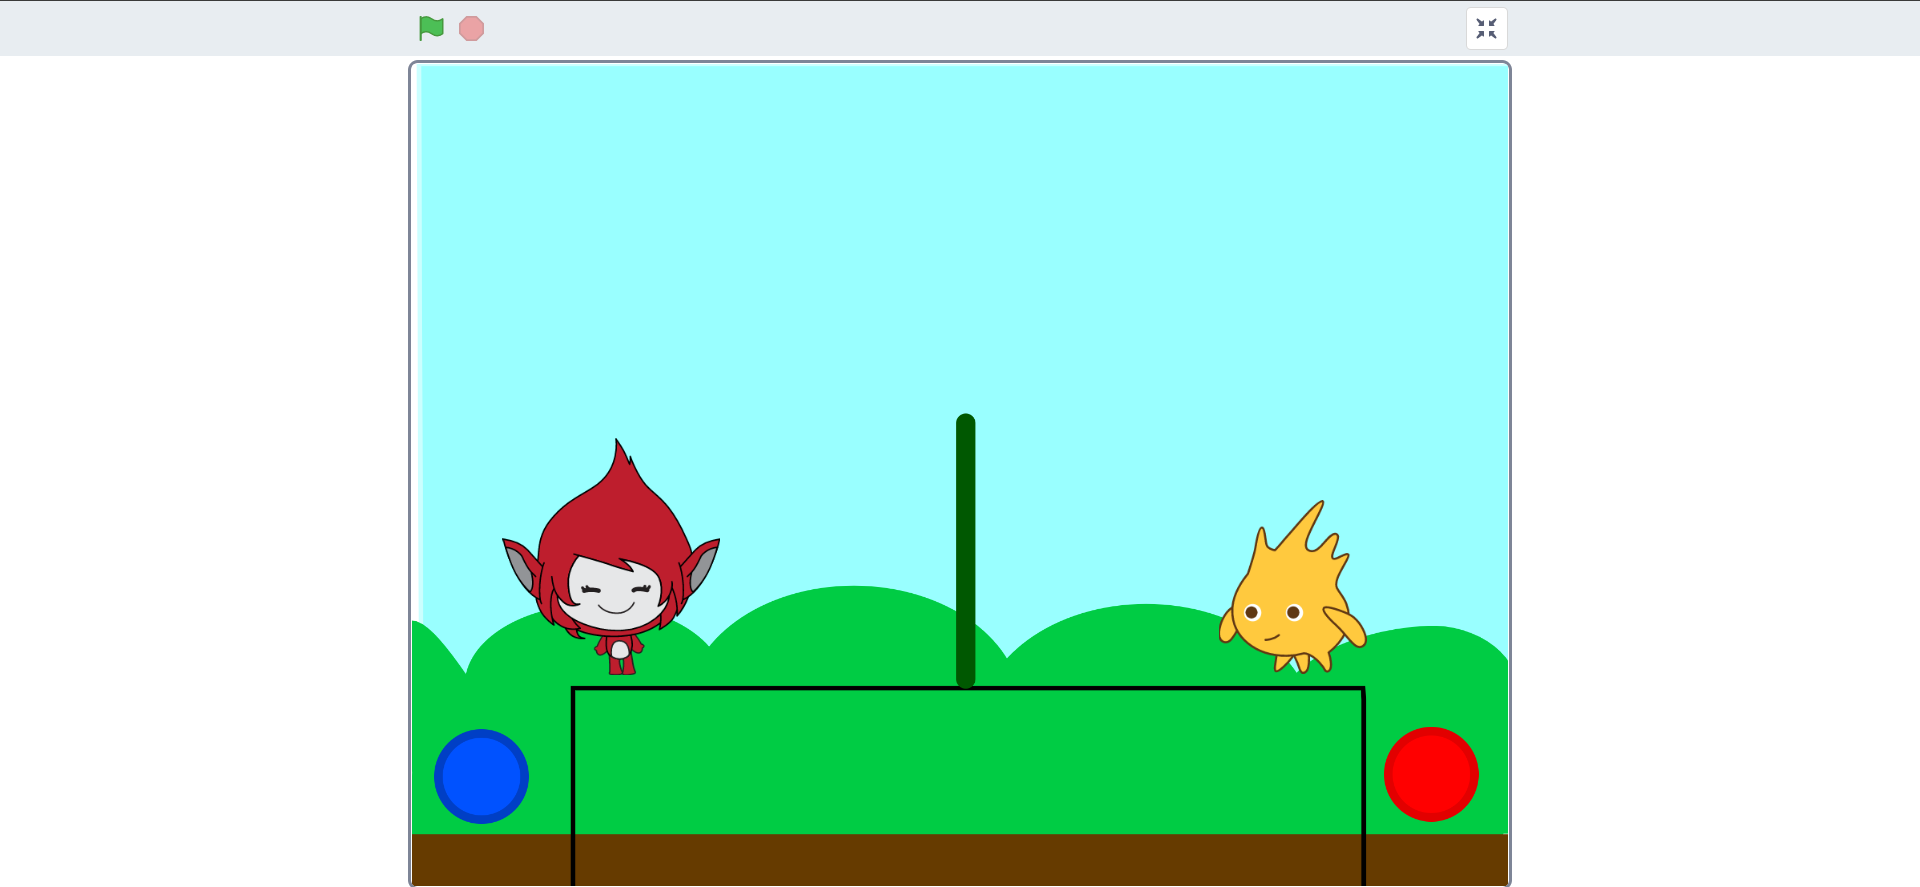
\includegraphics[width=1.0\linewidth,height=0.5\linewidth]{fig030001.png}
   \caption{Click and win}
\label{fig030001}
\end{figure}

\section{Adding Background and Characters}
Building the game starts with choosing a background. From the Backdrops->Choose a Backdrop section, a suitable one can be selected from the available ones that Scratch provides.

\begin{figure}[H]
   \centering
   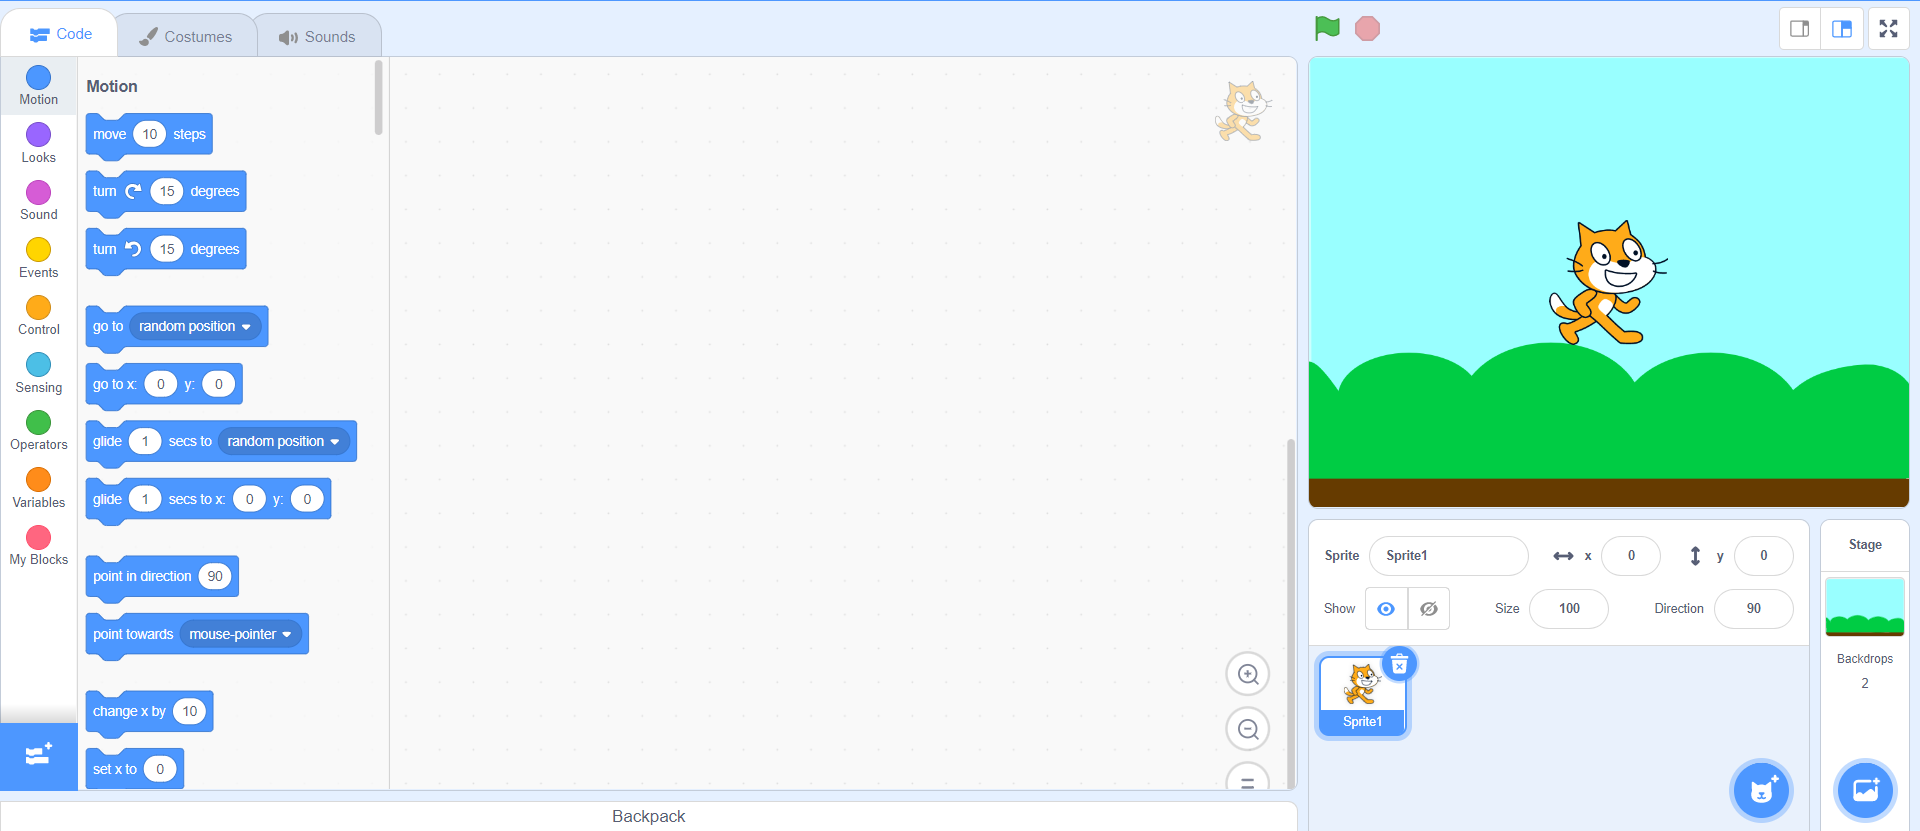
\includegraphics[width=1.0\linewidth,height=0.5\linewidth]{fig030002.png}
   \caption{Choosing a suitable background for the game}
\label{fig030002}
\end{figure}

In this dumbbell, to make the race course along with the green finish line, the background needs to be enhanced. For this purpose, the Backdrops option is first selected.

\begin{figure}[H]
   \centering
   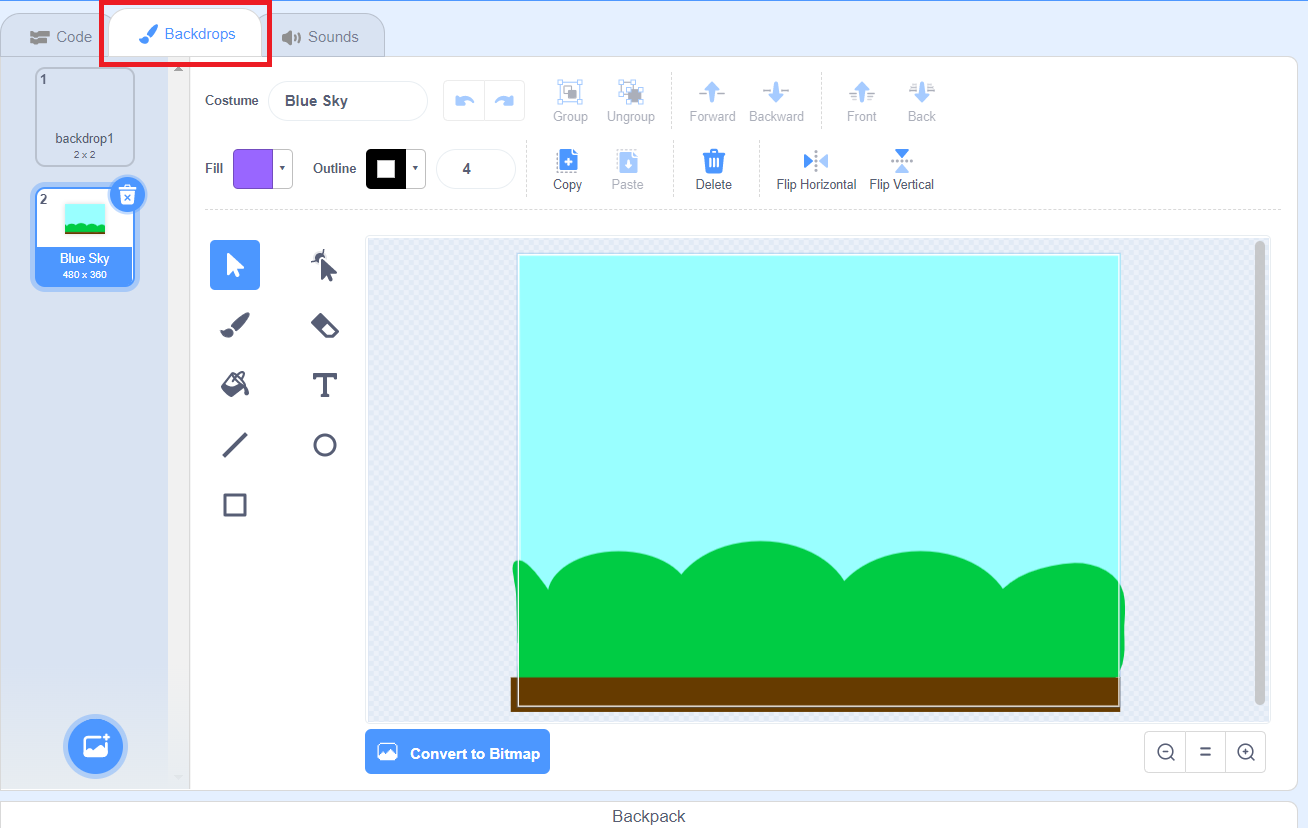
\includegraphics[width=1.0\linewidth,height=0.5\linewidth]{fig030003.png}
   \caption{Drawing additional elements on the background}
\label{fig030003}
\end{figure}

Using the line tool, the race track is added. If the thickness and color of the line is changed, the finish line can also be added.

\begin{figure}[H]
   \centering
   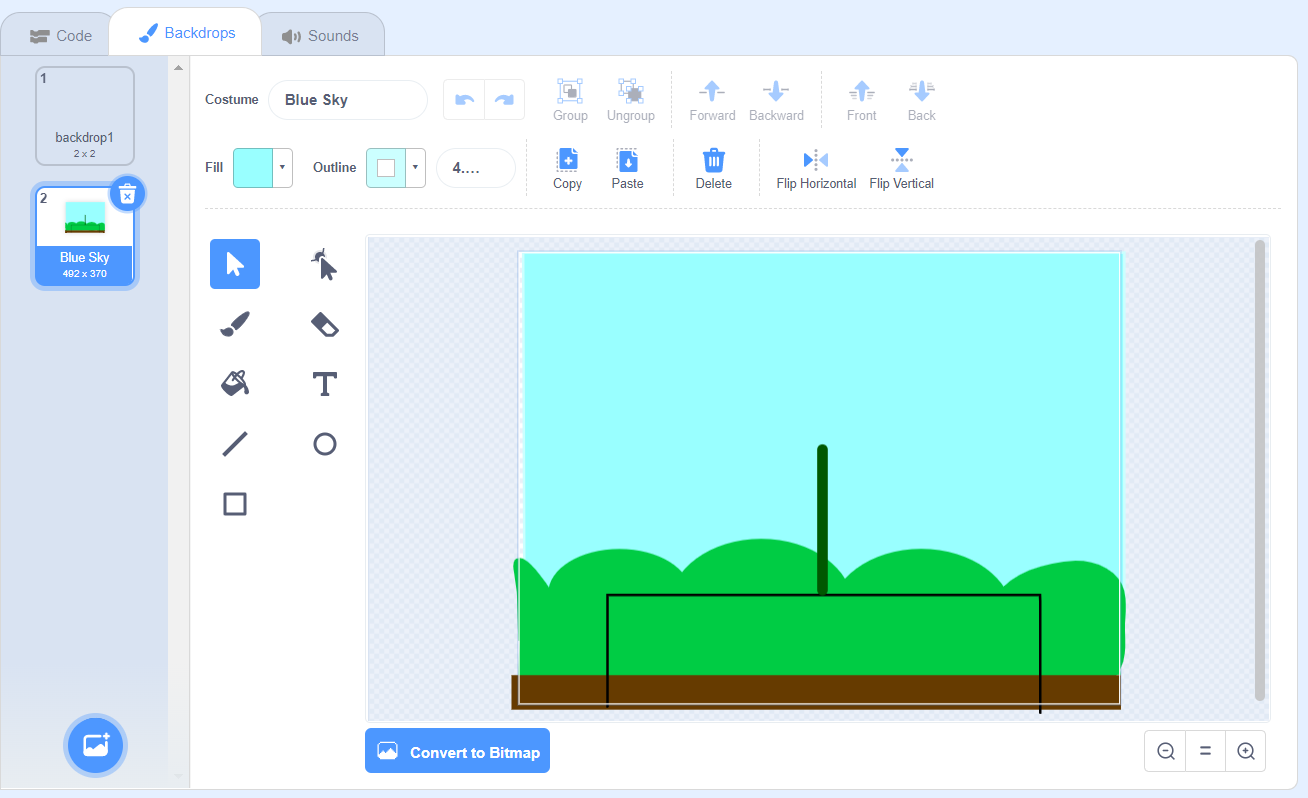
\includegraphics[width=1.0\linewidth,height=0.5\linewidth]{fig030004.png}
   \caption{Final Game Background}
\label{fig030004}
\end{figure}

If the game does not need the main character in the Scratch cat, he can be deleted.

\begin{figure}[H]
   \centering
   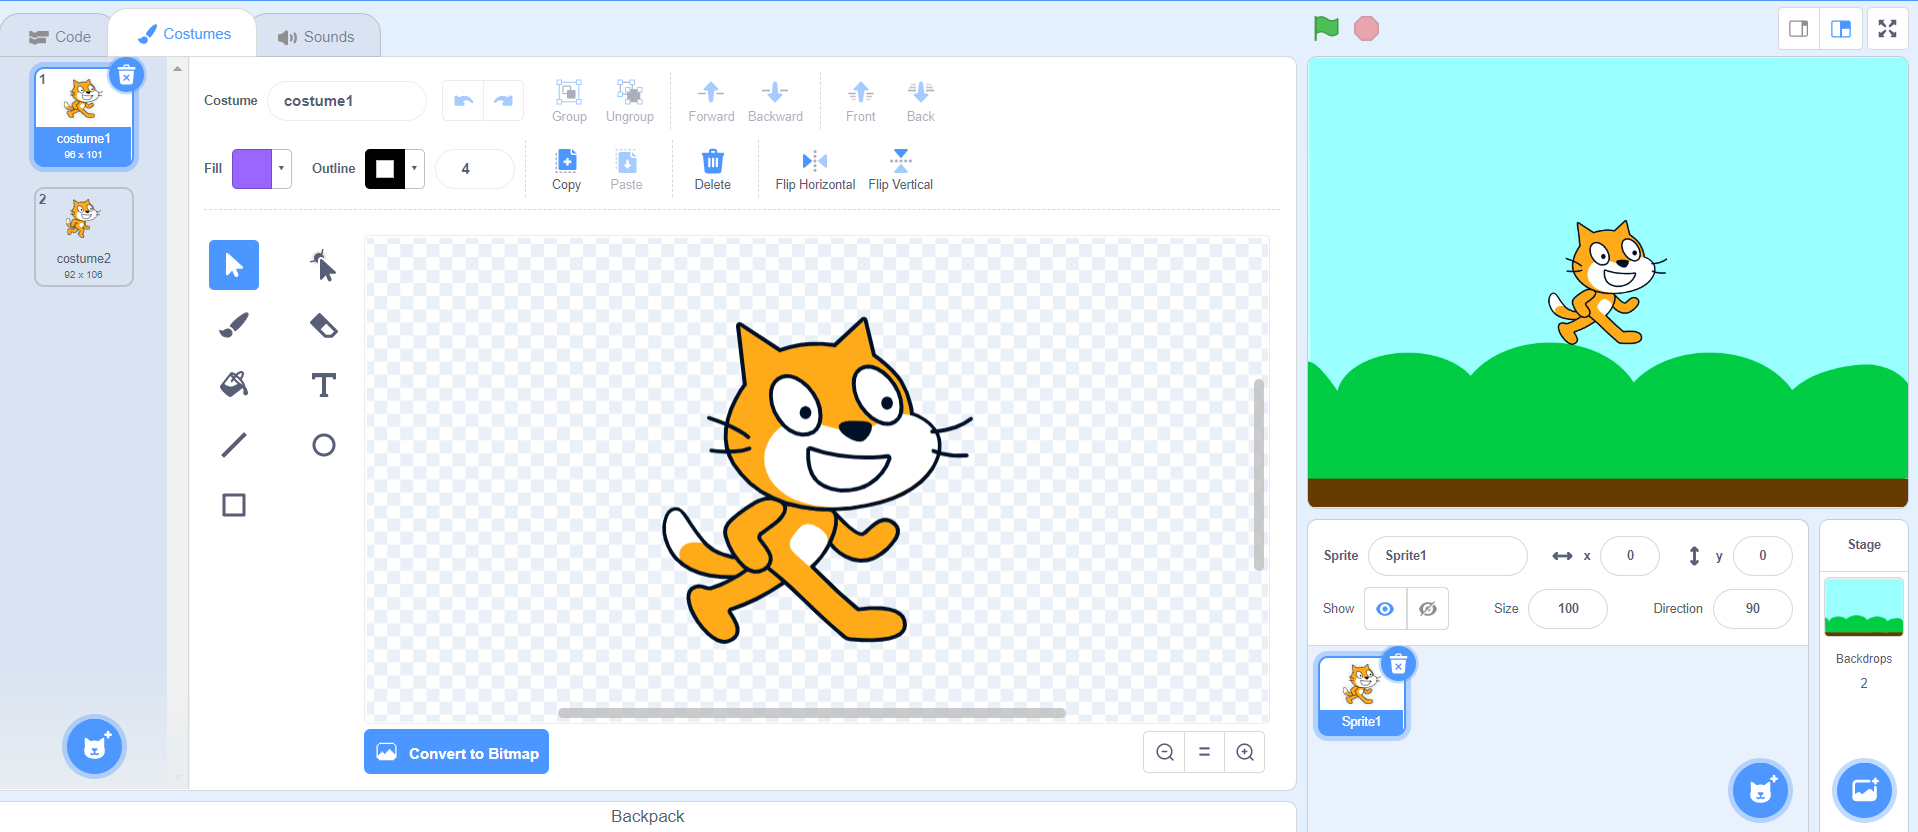
\includegraphics[width=1.0\linewidth,height=0.5\linewidth]{fig030005.png}
   \caption{Delete main character}
\label{fig030005}
\end{figure}

The characters should also be added to the game. There are many sprites available in Scratch. For the purposes of this game, two are needed - one that is positioned on the left and one on the right (Fig. \ref{fig030006}). The Size and Direction properties change the size and direction of the character.

\begin{figure}[H]
   \centering
   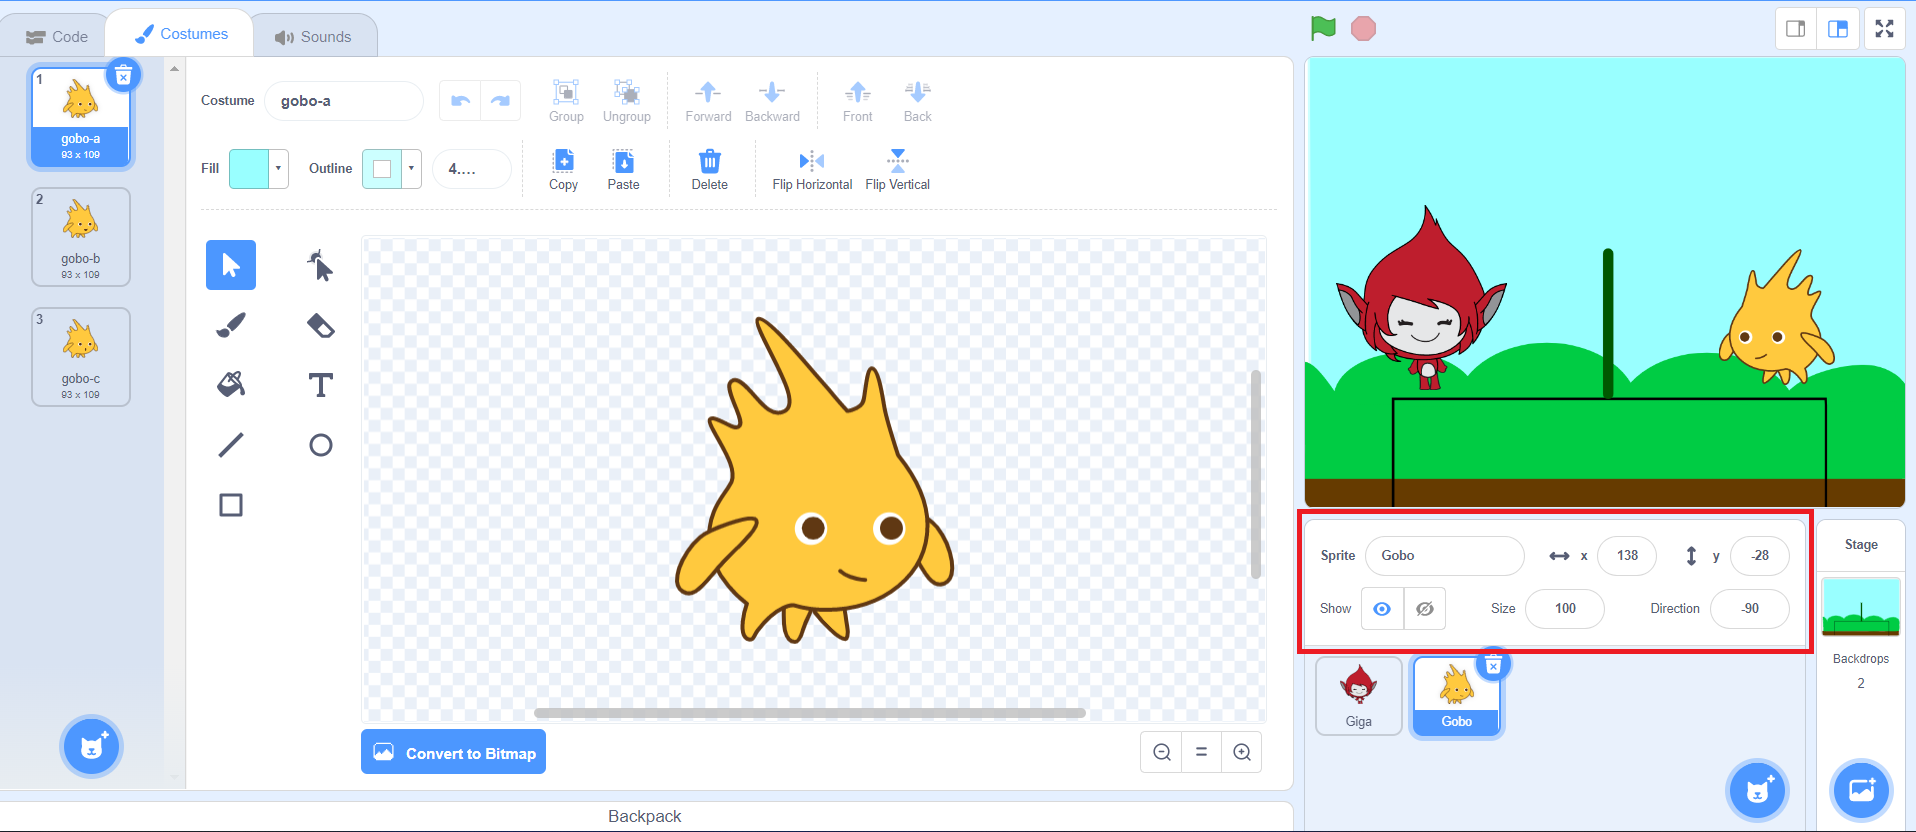
\includegraphics[width=1.0\linewidth,height=0.5\linewidth]{fig030006.png}
   \caption{In-Game Characters}
\label{fig030006}
\end{figure}

In addition to these two sprites, two more are needed, which are the buttons that the players must click on. They are found again in the Sprite section. In this game, the buttons must be a different color to differentiate them. To change the color of a button, it must change its suit.

\begin{figure}[H]
   \centering
   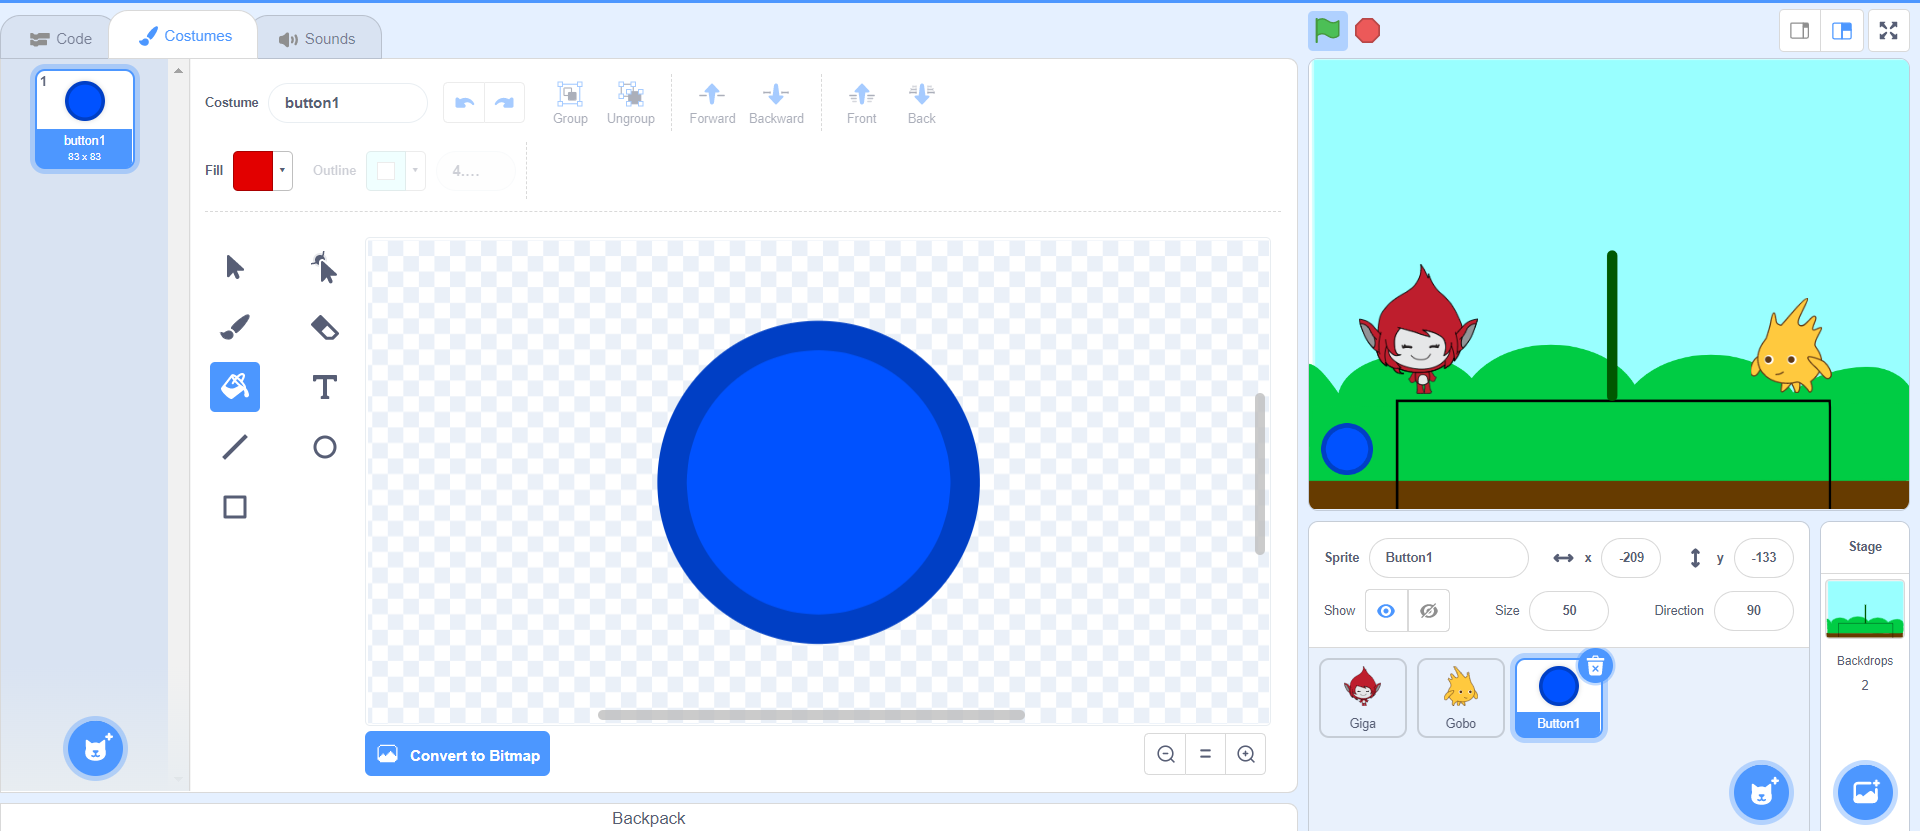
\includegraphics[width=1.0\linewidth,height=0.5\linewidth]{fig030007.png}
   \caption{Blue Button}
\label{fig030007}
\end{figure}

Using the Fill tool, change the color of the button (Fig. \ref{fig030008}). The same can be done for the red button. Again, the Size property can change the size of this sprite.

\begin{figure}[H]
   \centering
   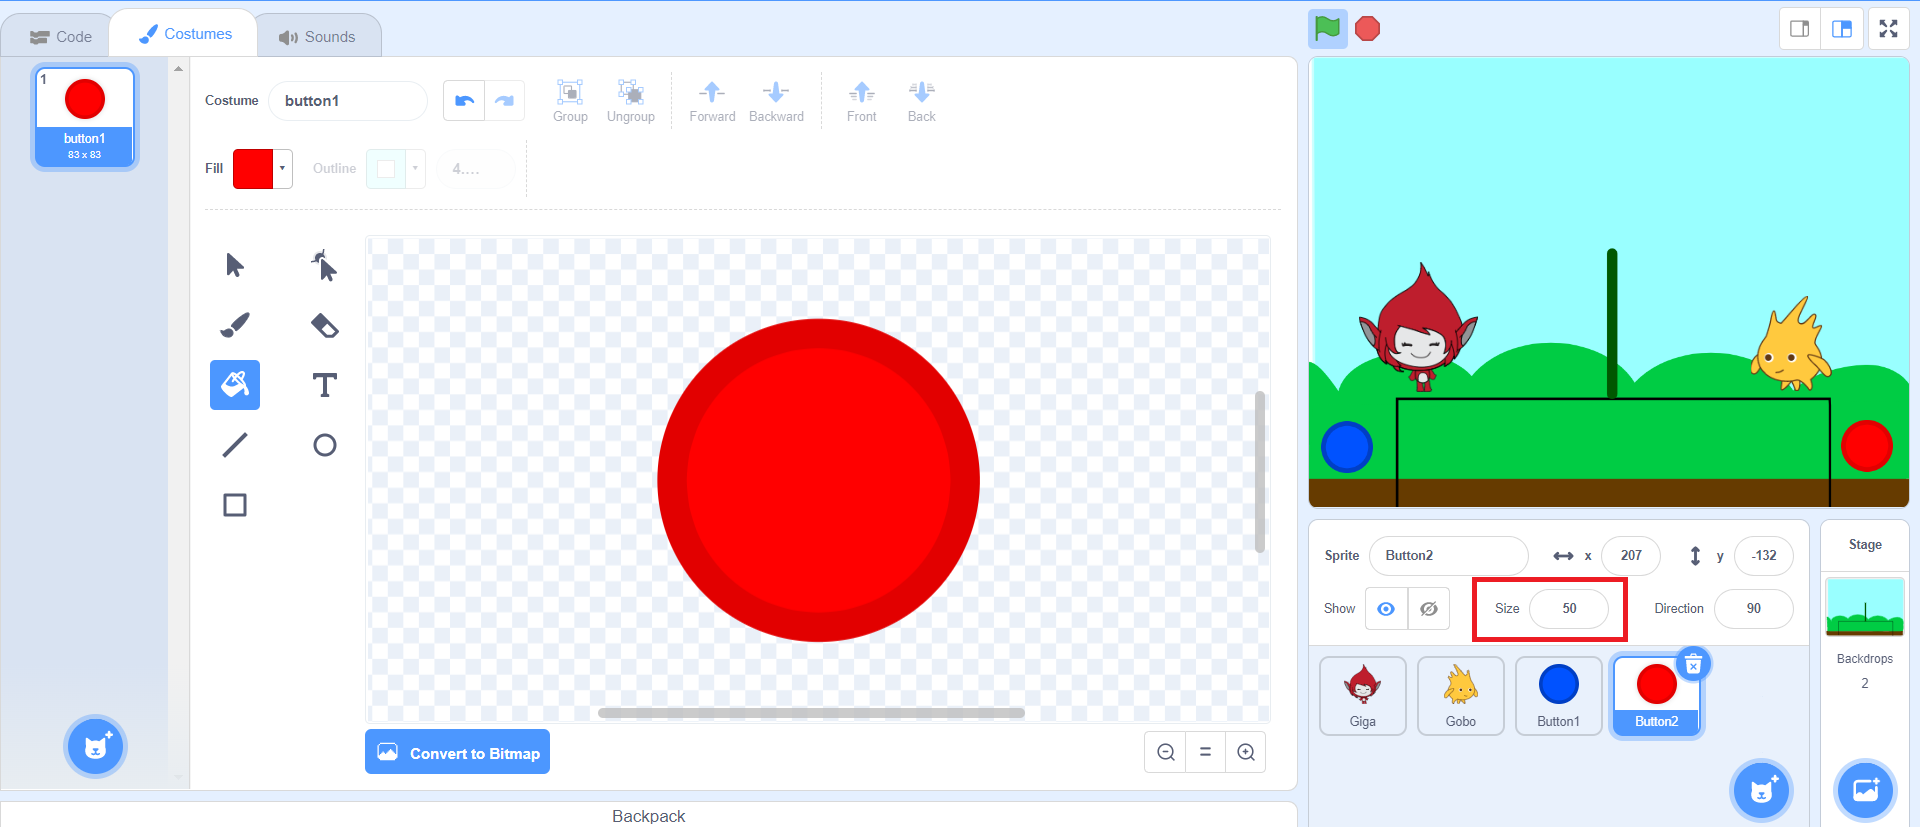
\includegraphics[width=1.0\linewidth,height=0.5\linewidth]{fig030008.png}
   \caption{Red Button}
\label{fig030008}
\end{figure}

\section{Blue Button Programming}
When the player clicks on the blue button, it should send a message "blue". The first starting block to be placed is when this sprite is clicked.

\begin{figure}[H]
   \centering
   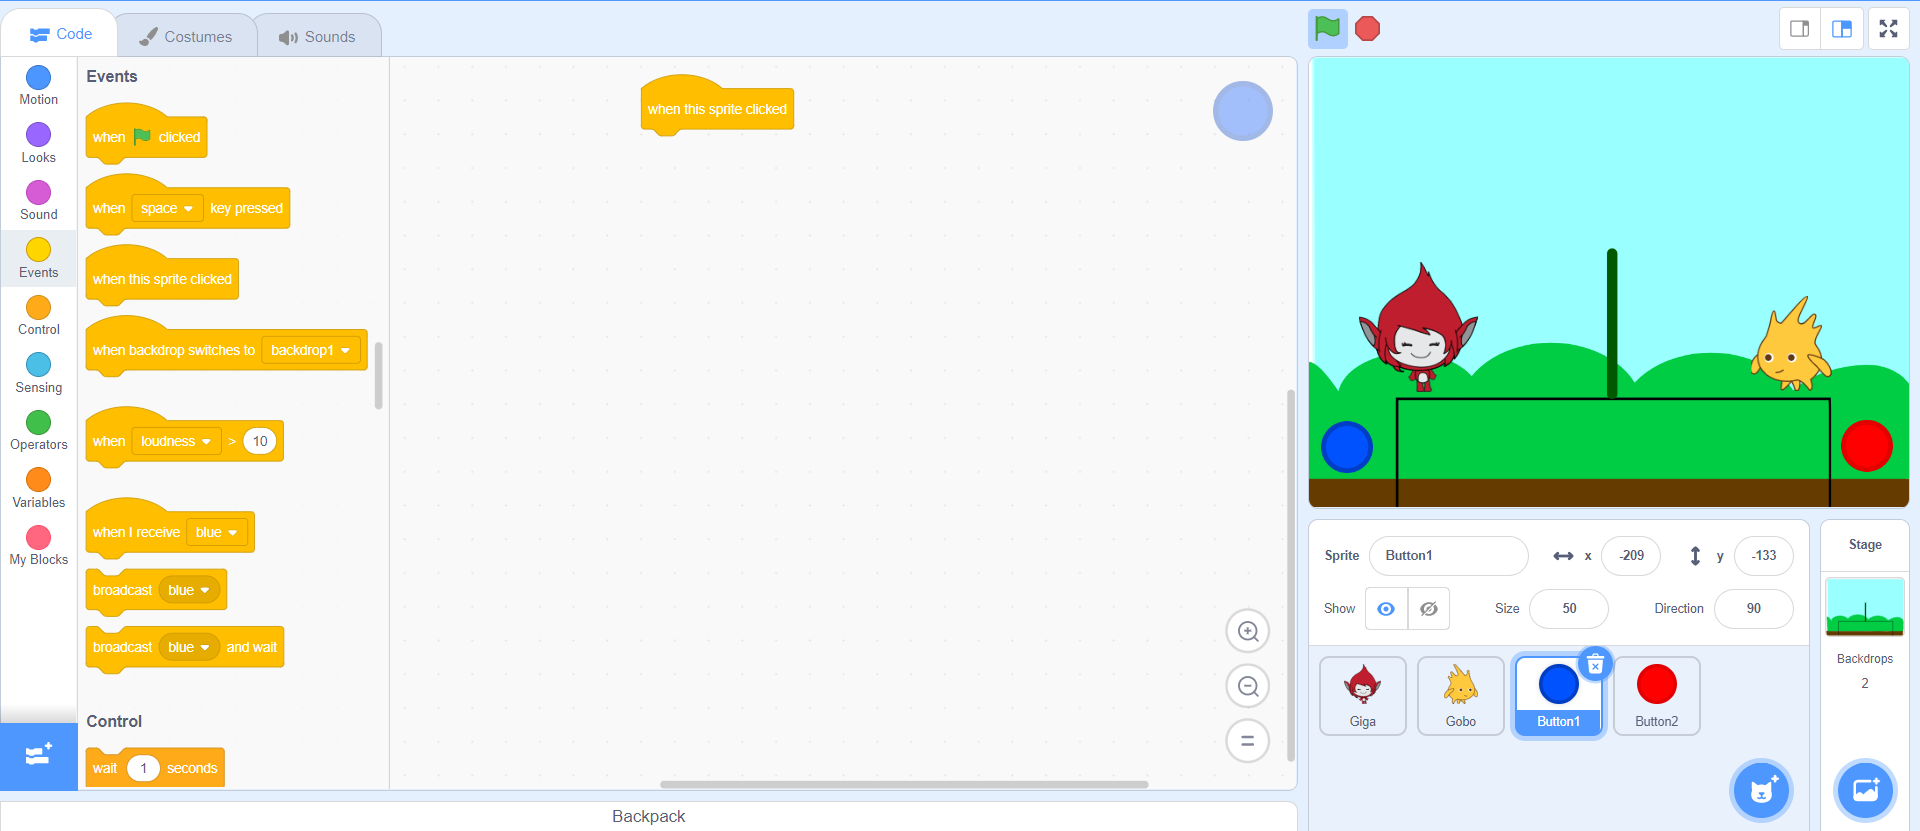
\includegraphics[width=1.0\linewidth,height=0.5\linewidth]{fig030009.png}
   \caption{When character is clicked}
\label{fig030009}
\end{figure}

Next, the character sends a "blue" message. From the dark orange group the message propagation instruction. The message to spread is "blue".

\begin{figure}[H]
   \centering
   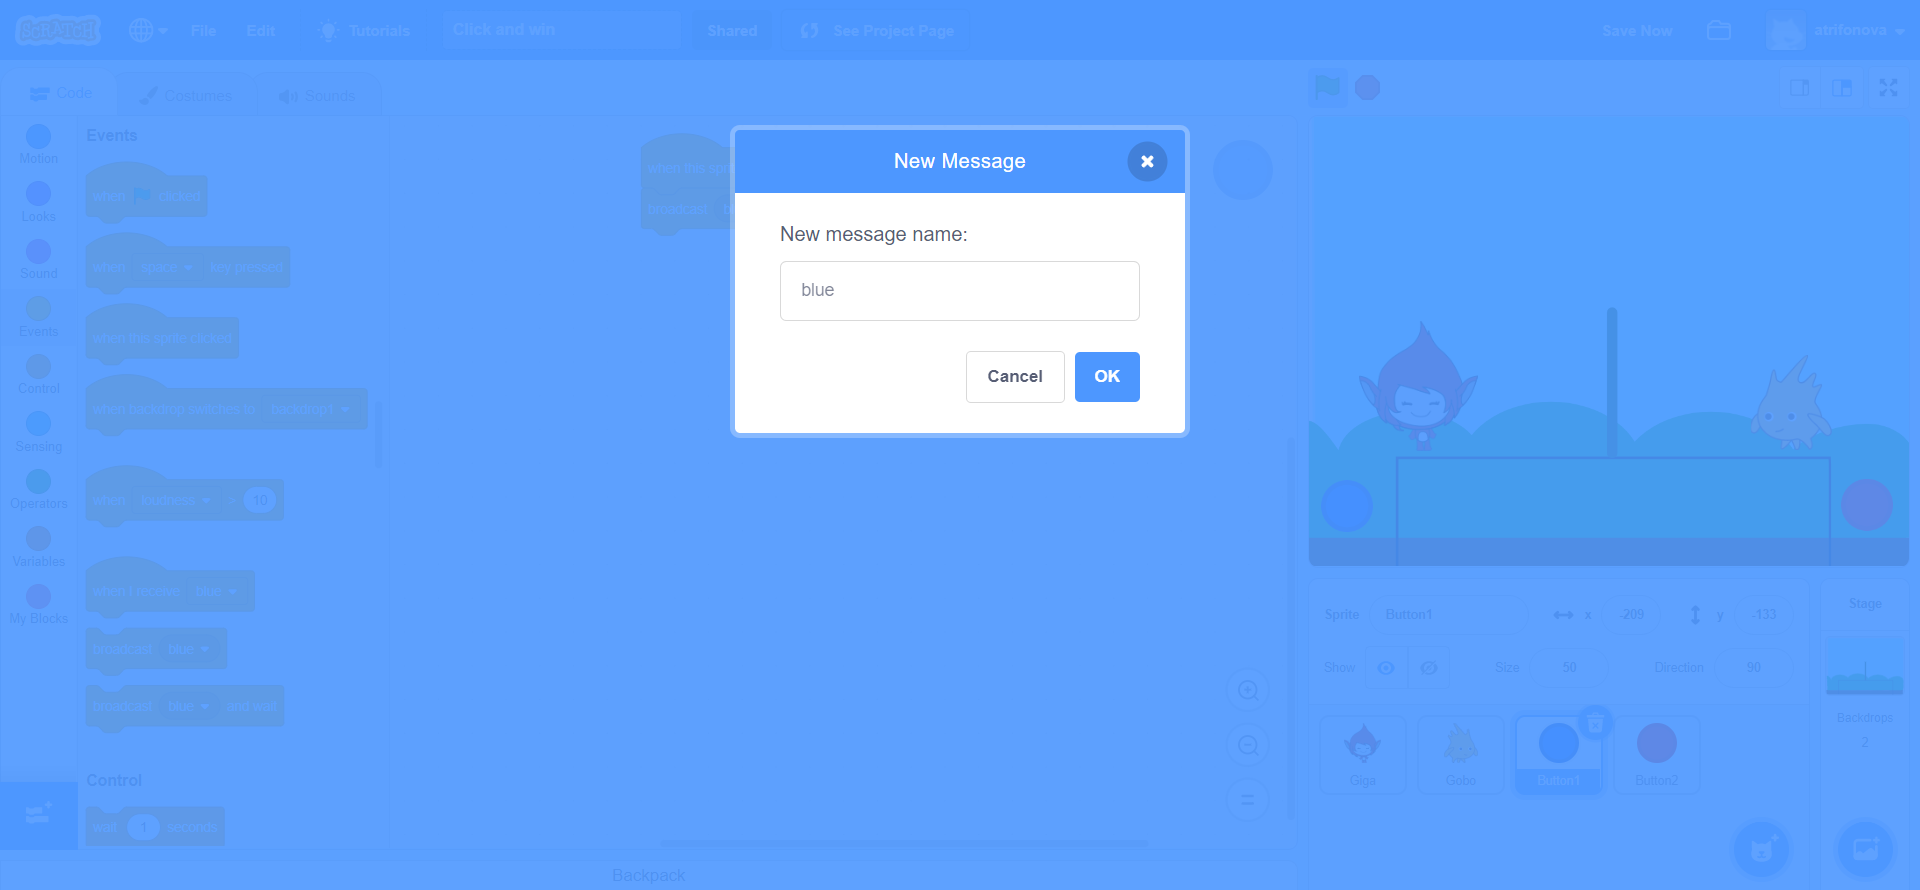
\includegraphics[width=1.0\linewidth,height=0.5\linewidth]{fig030010.png}
   \caption{Send Message}
\label{fig030010}
\end{figure}

The code for this character looks like this:

\begin{figure}[H]
   \centering
   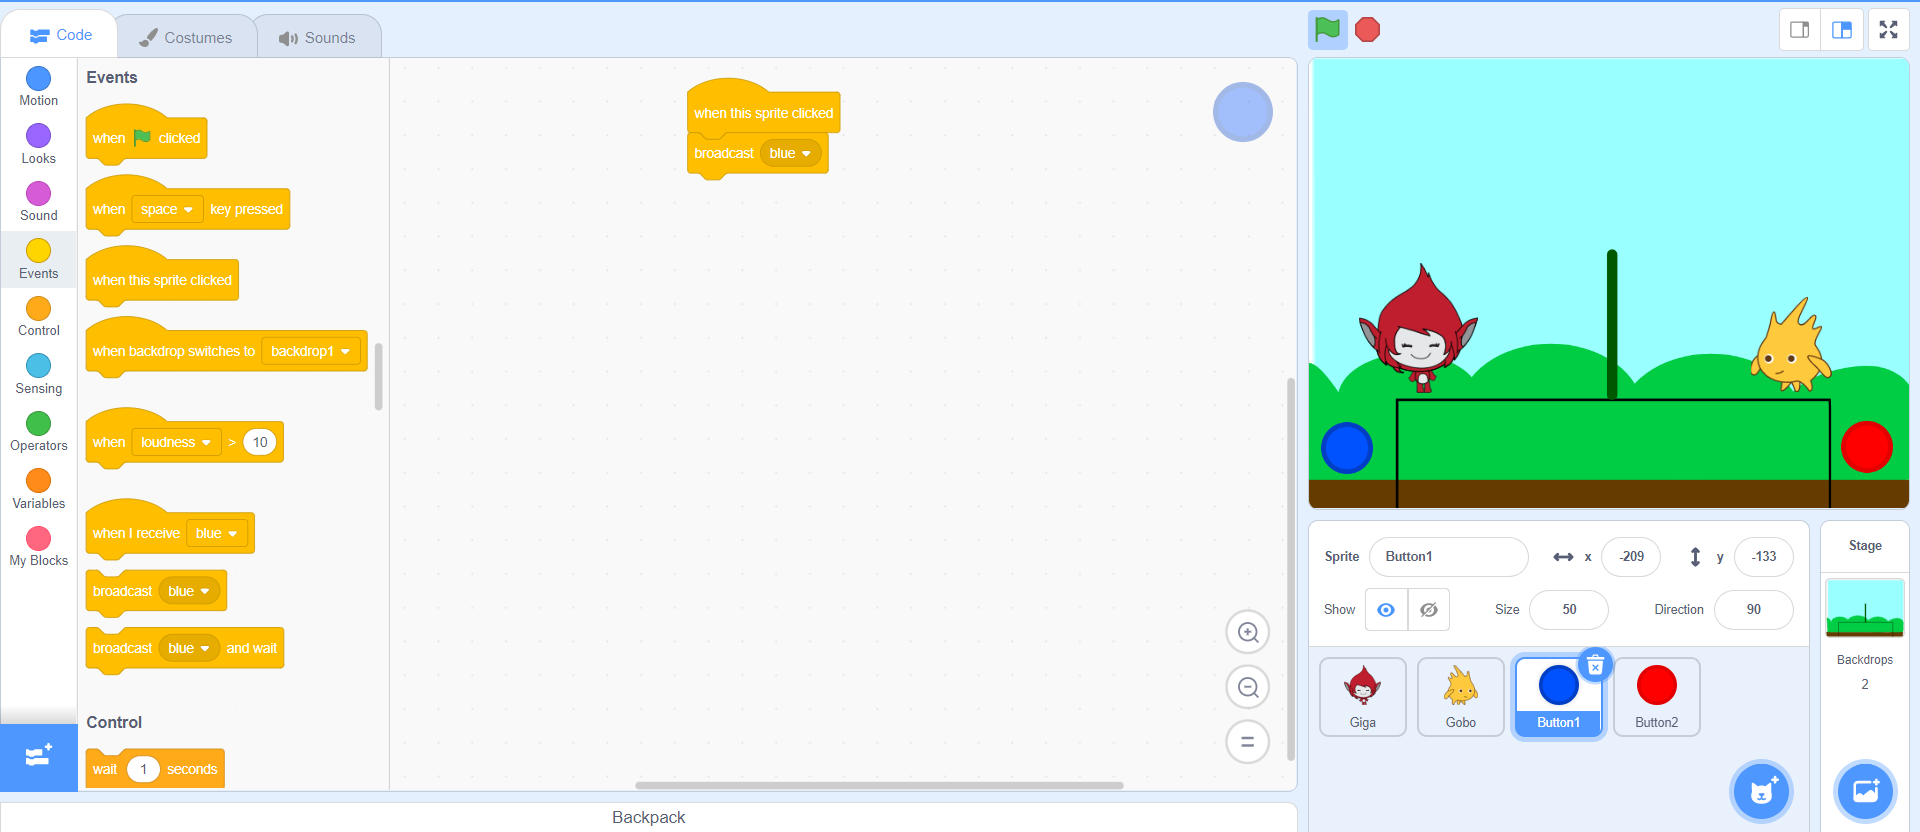
\includegraphics[width=1.0\linewidth,height=0.5\linewidth]{fig030011.png}
   \caption{The entire blue button code}
\label{fig030011}
\end{figure}

\section{Programming the Red Button}
When the player clicks on the red button, similarly to the blue one, it should send a "red" message. The code for the red button is as follows:

\begin{figure}[H]
   \centering
   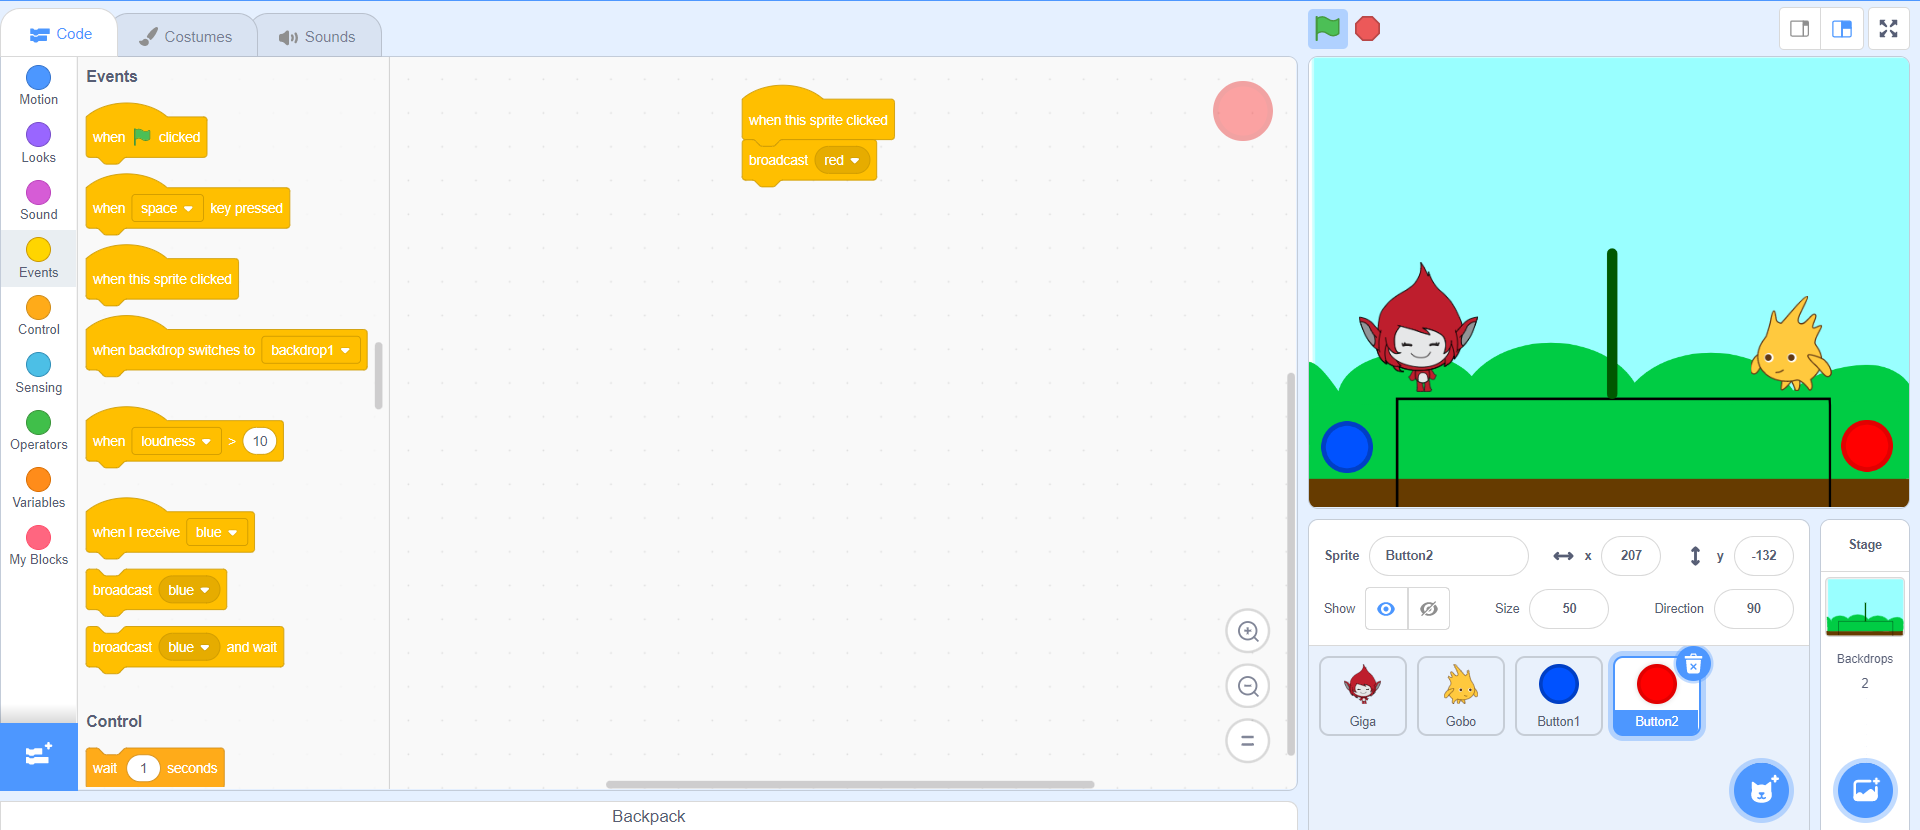
\includegraphics[width=1.0\linewidth,height=0.5\linewidth]{fig030012.png}
   \caption{All red button code}
\label{fig030012}
\end{figure}

Up to this point, the program consists of when the player presses the blue or red button, they send the corresponding messages.

\section{Programming characters to move}
The instructions on the blue button are that it sends a message. The left character must subscribe to receive the message.

\begin{figure}[H]
   \centering
   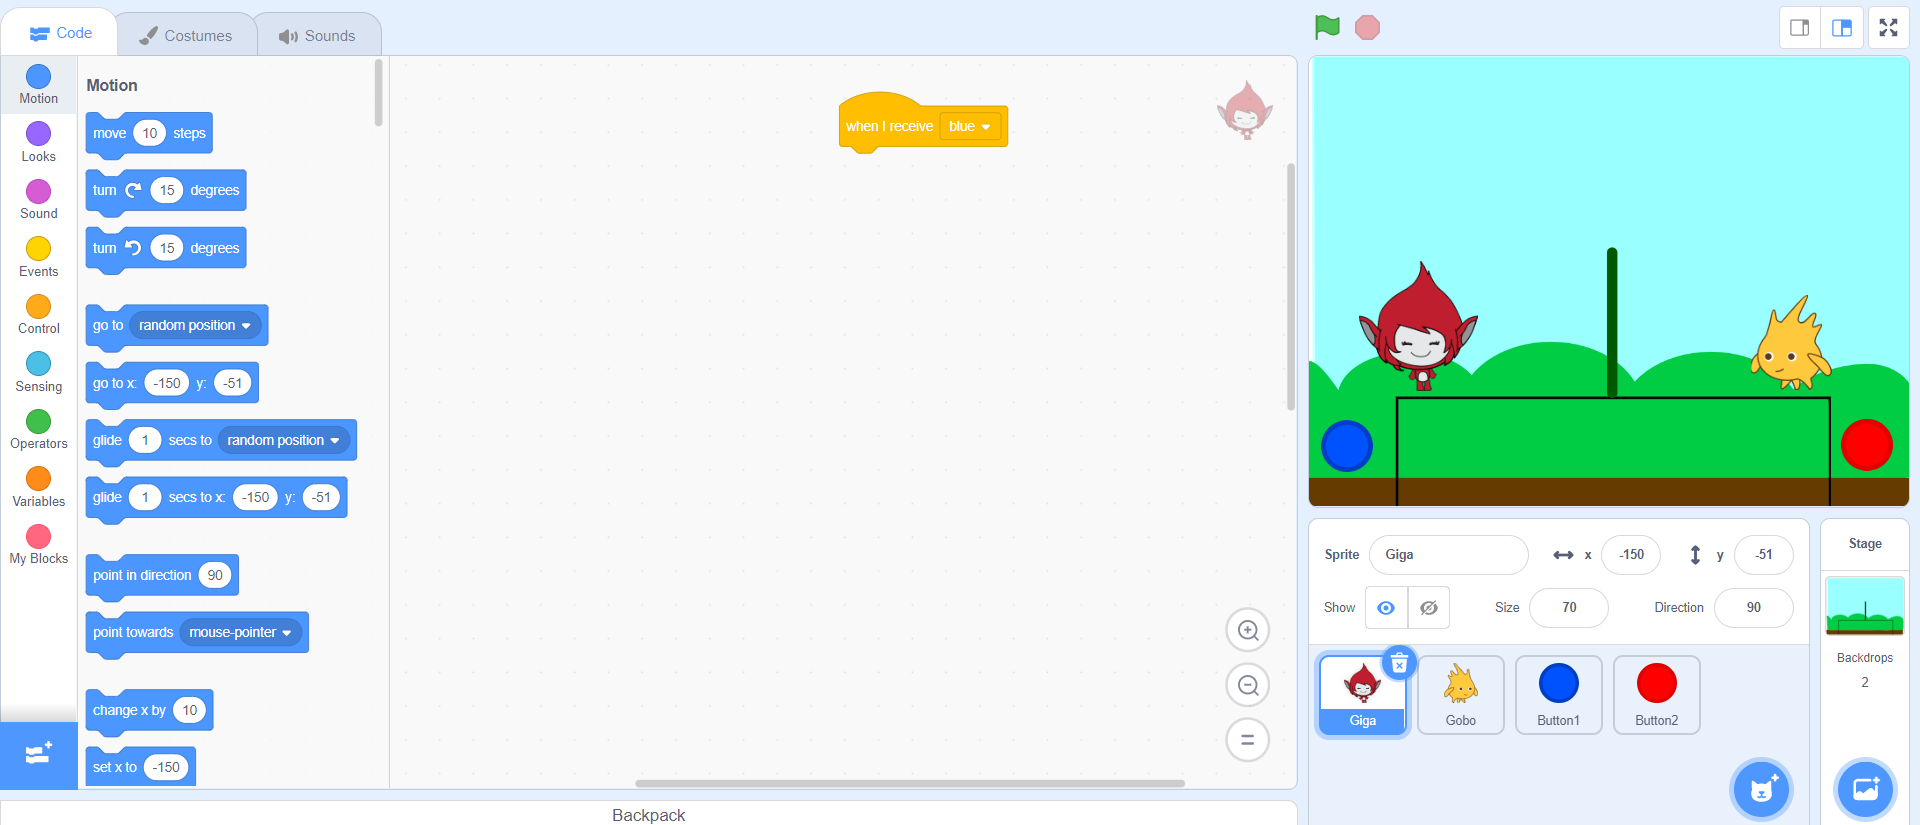
\includegraphics[width=1.0\linewidth,height=0.5\linewidth]{fig030013.png}
   \caption{Subscribe to the message from the blue button}
\label{fig030013}
\end{figure}

The character must move right to the green finish line, which means the x coordinate must be changed, increasing it by 3 steps.

\begin{figure}[H]
\centering
   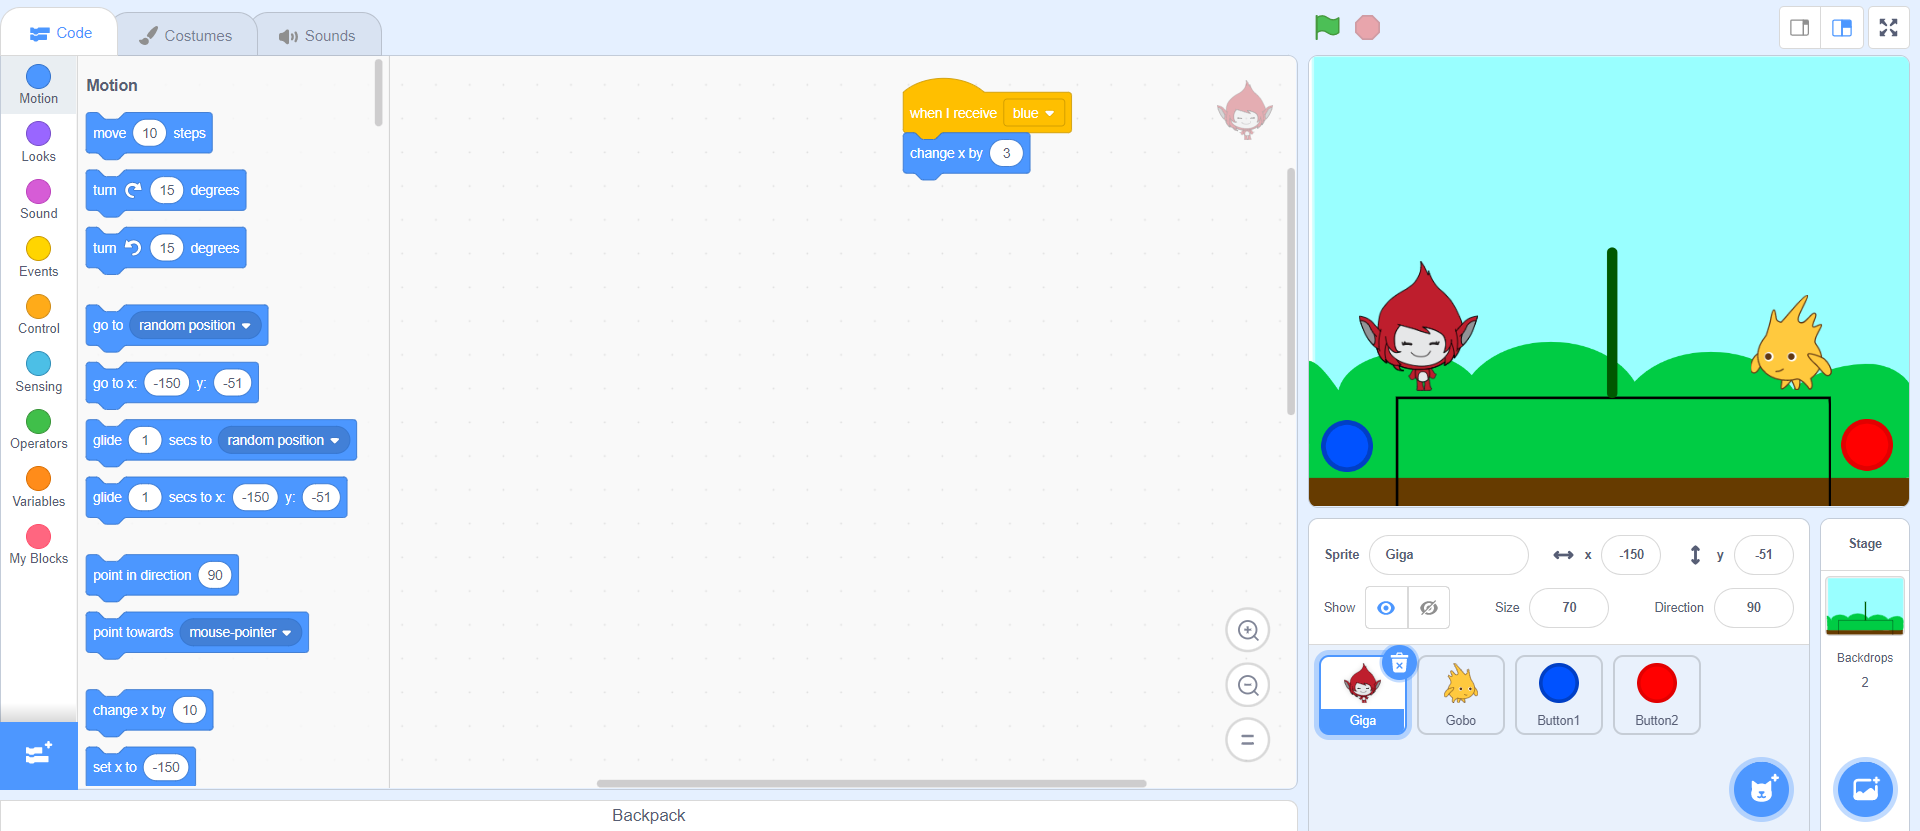
\includegraphics[width=1.0\linewidth,height=0.5\linewidth]{fig030014.png}
   \caption{Move Character Right}
\label{fig030014}
\end{figure}

The instructions for the other character are similar. The main differences are two:
- the message this character subscribes to was sent by the red button
- the character must move left towards the green finish line, which means the x coordinate must be changed, decreasing it by 3 steps

\begin{figure}[H]
   \centering
   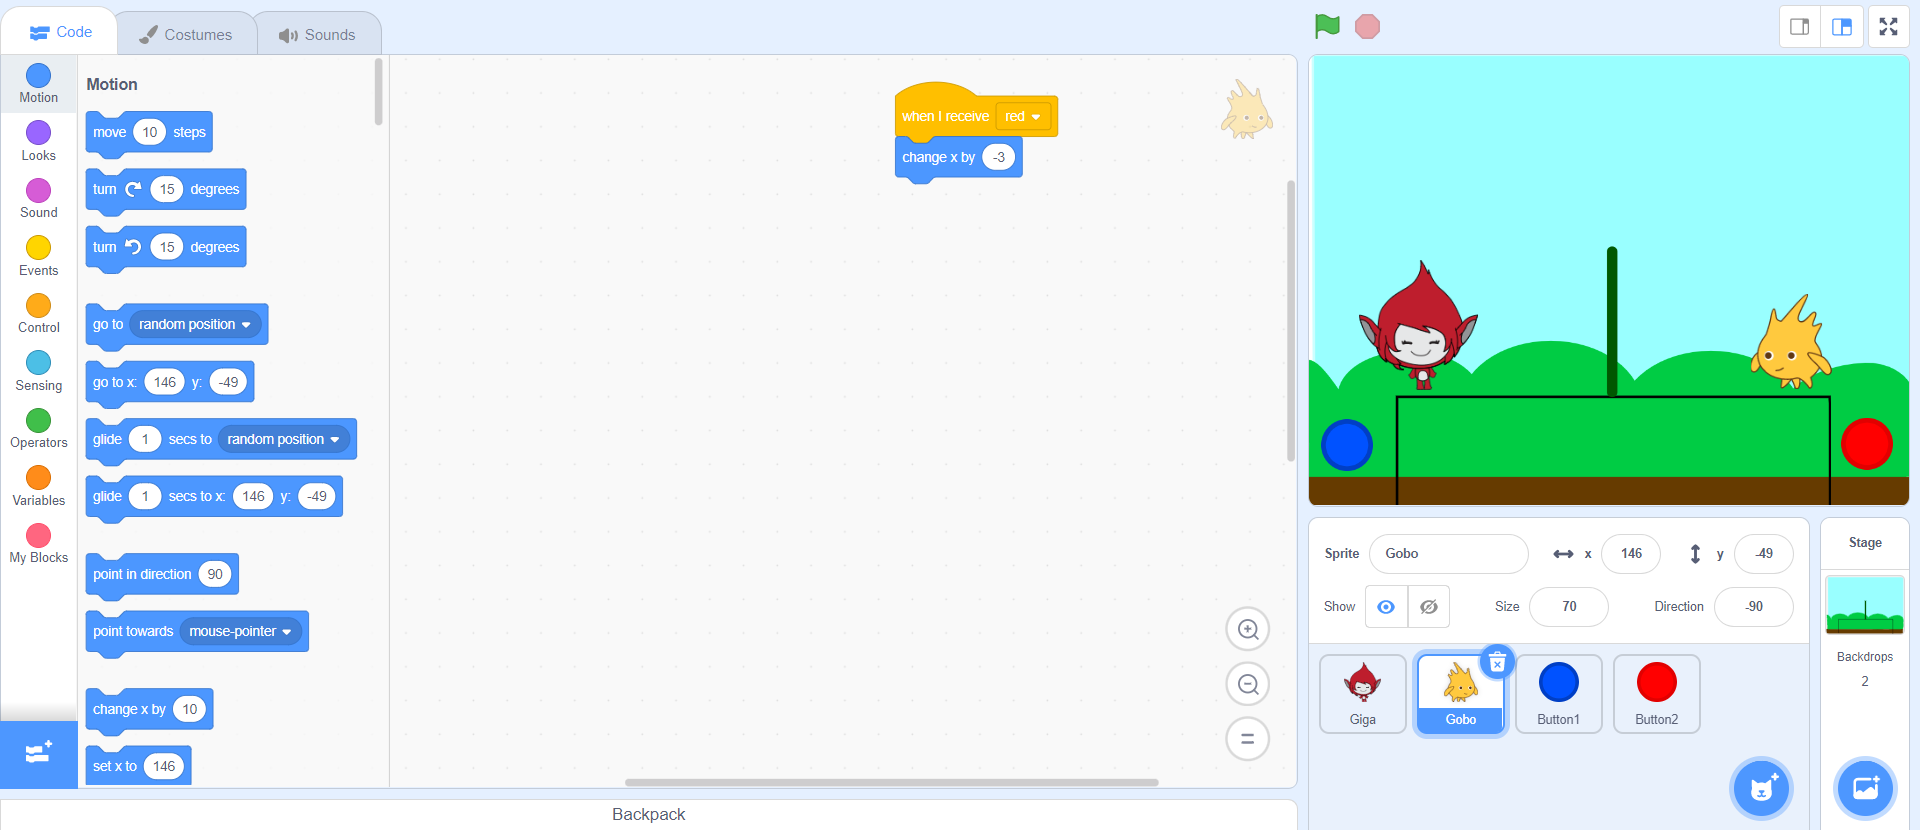
\includegraphics[width=1.0\linewidth,height=0.5\linewidth]{fig030015.png}
   \caption{Move Character Left}
\label{fig030015}
\end{figure}

\section{Programming the winner}
To complete the game, it remains to check which of the characters has reached the green finish line.

In the right character, the first instruction to add is the initial to start the game. At each moment of the game, it must be checked whether the character has reached the finish line. For this reason, a forever loop instruction must be added.

\begin{figure}[H]
   \centering
   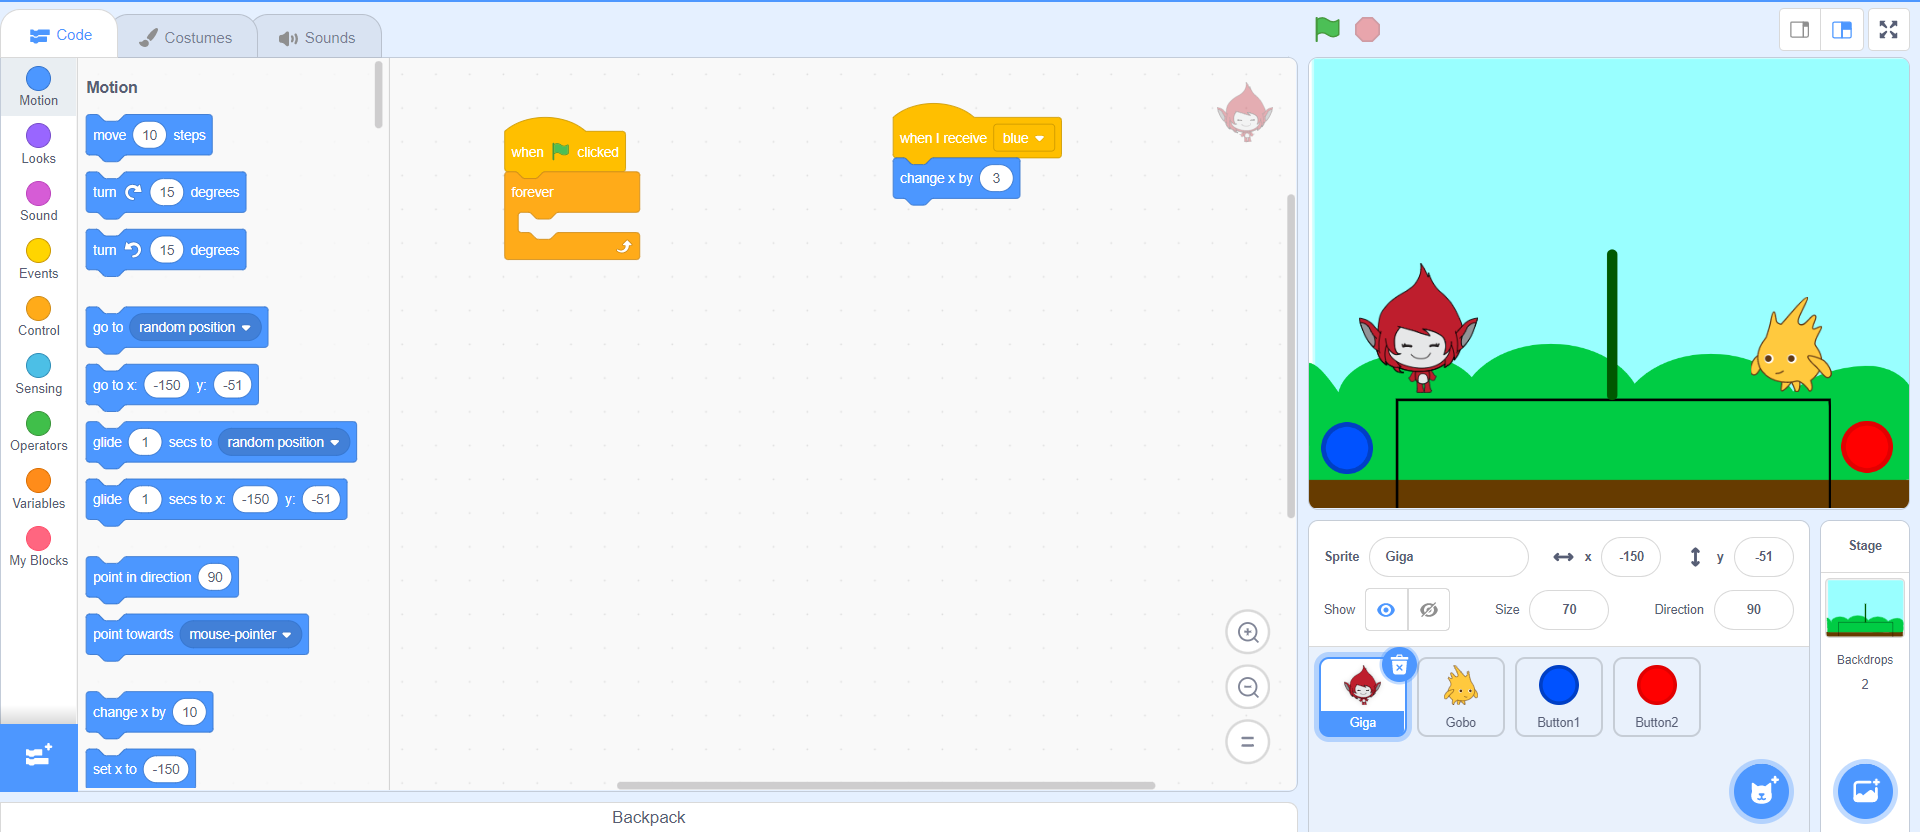
\includegraphics[width=1.0\linewidth,height=0.5\linewidth]{fig030016.png}
   \caption{Cycle Forever}
\label{fig030016}
\end{figure}

Inside the body of the loop should be the check to see if the character has touched the finish line.

\begin{figure}[H]
   \centering
   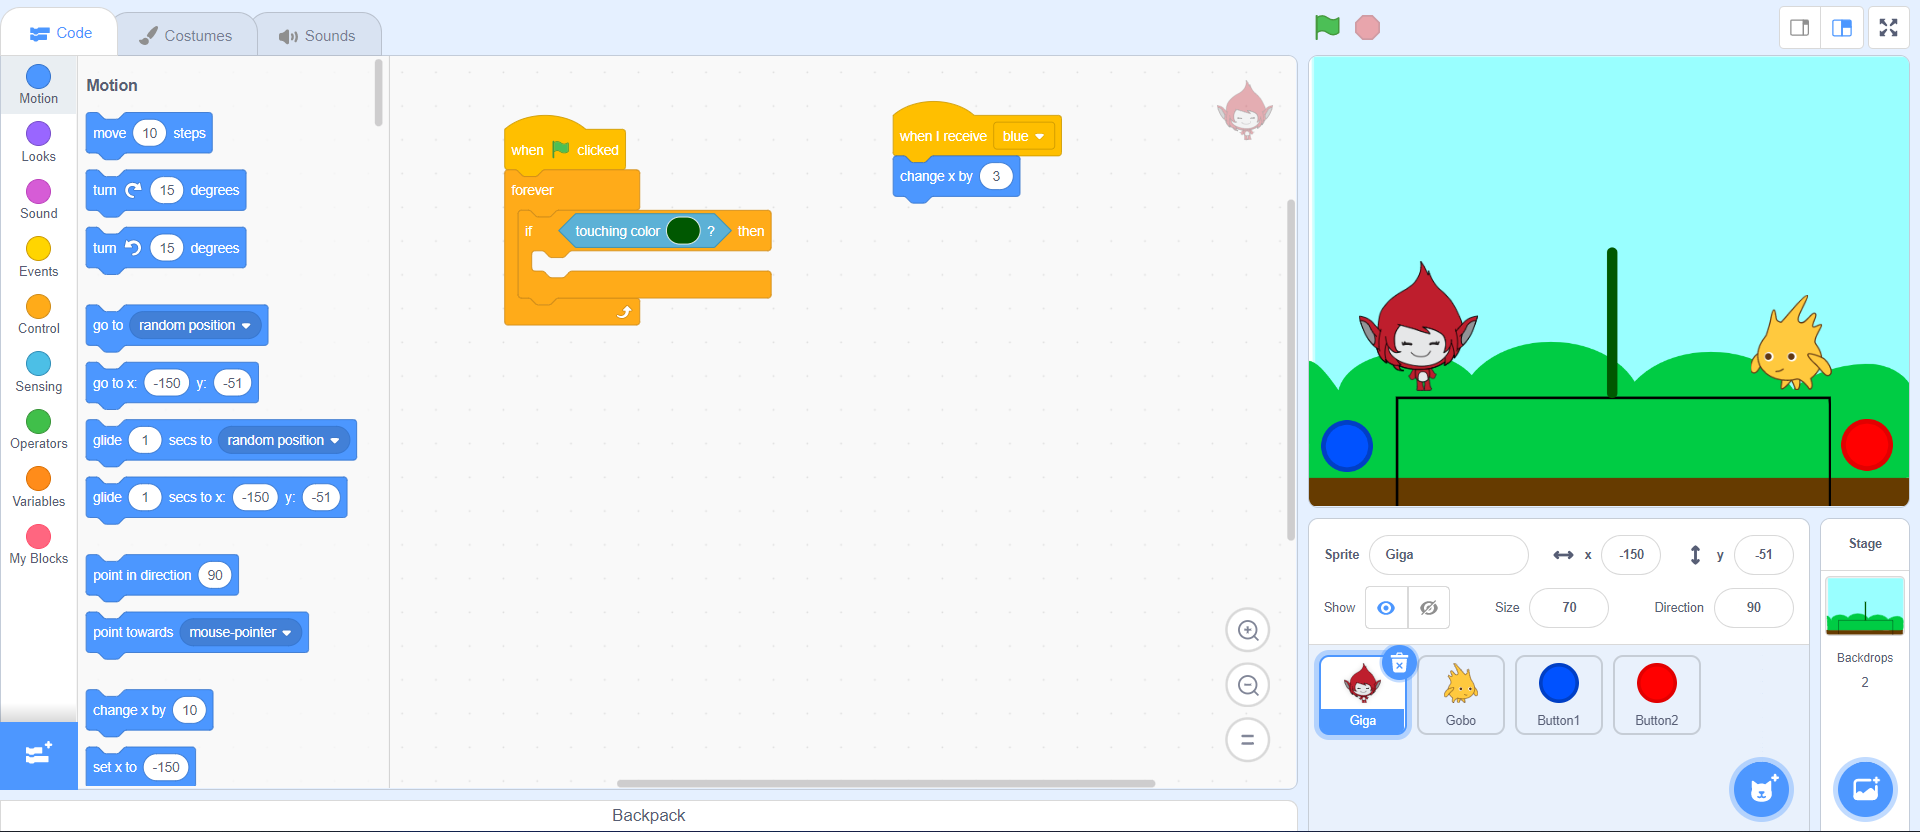
\includegraphics[width=1.0\linewidth,height=0.5\linewidth]{fig030017.png}
   \caption{Checking if character has reached finish}
\label{fig030017}
\end{figure}

To select the same green color as the finish line, the eyedropper tool should be used.

\begin{figure}[H]
   \centering
   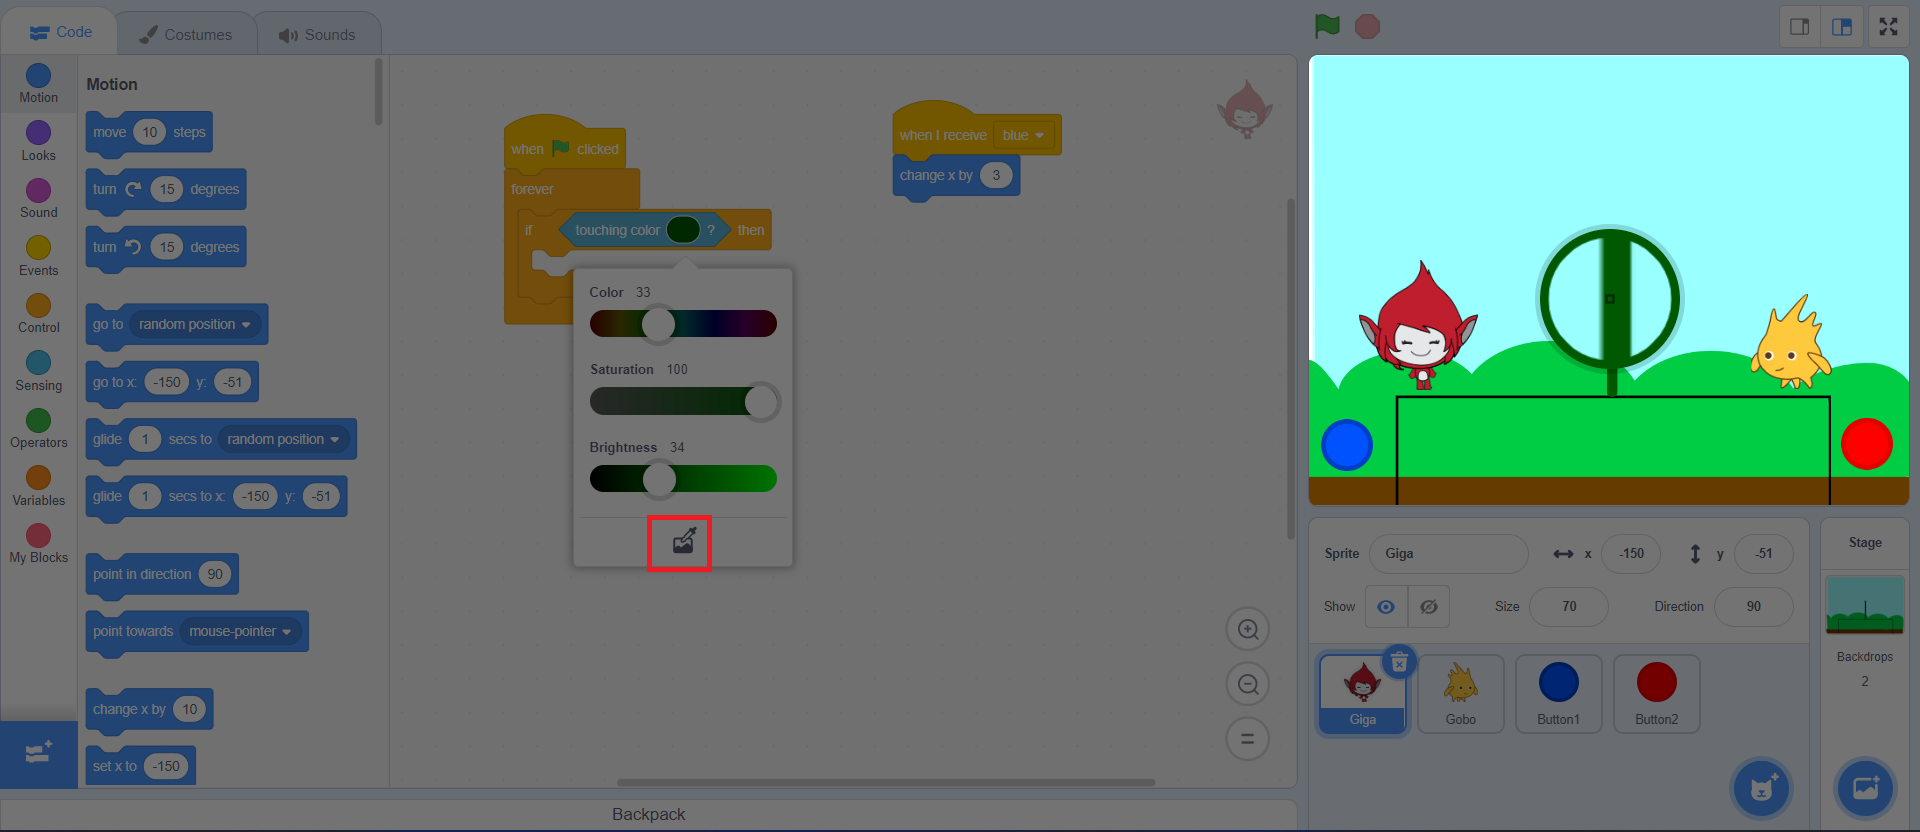
\includegraphics[width=1.0\linewidth,height=0.5\linewidth]{fig030018.png}
   \caption{Choose a color}
\label{fig030018}
\end{figure}

The instructions that are inside the condition will be executed when the character wins. Then he should increase his size and write a message "I won!".

\begin{figure}[H]
   \centering
   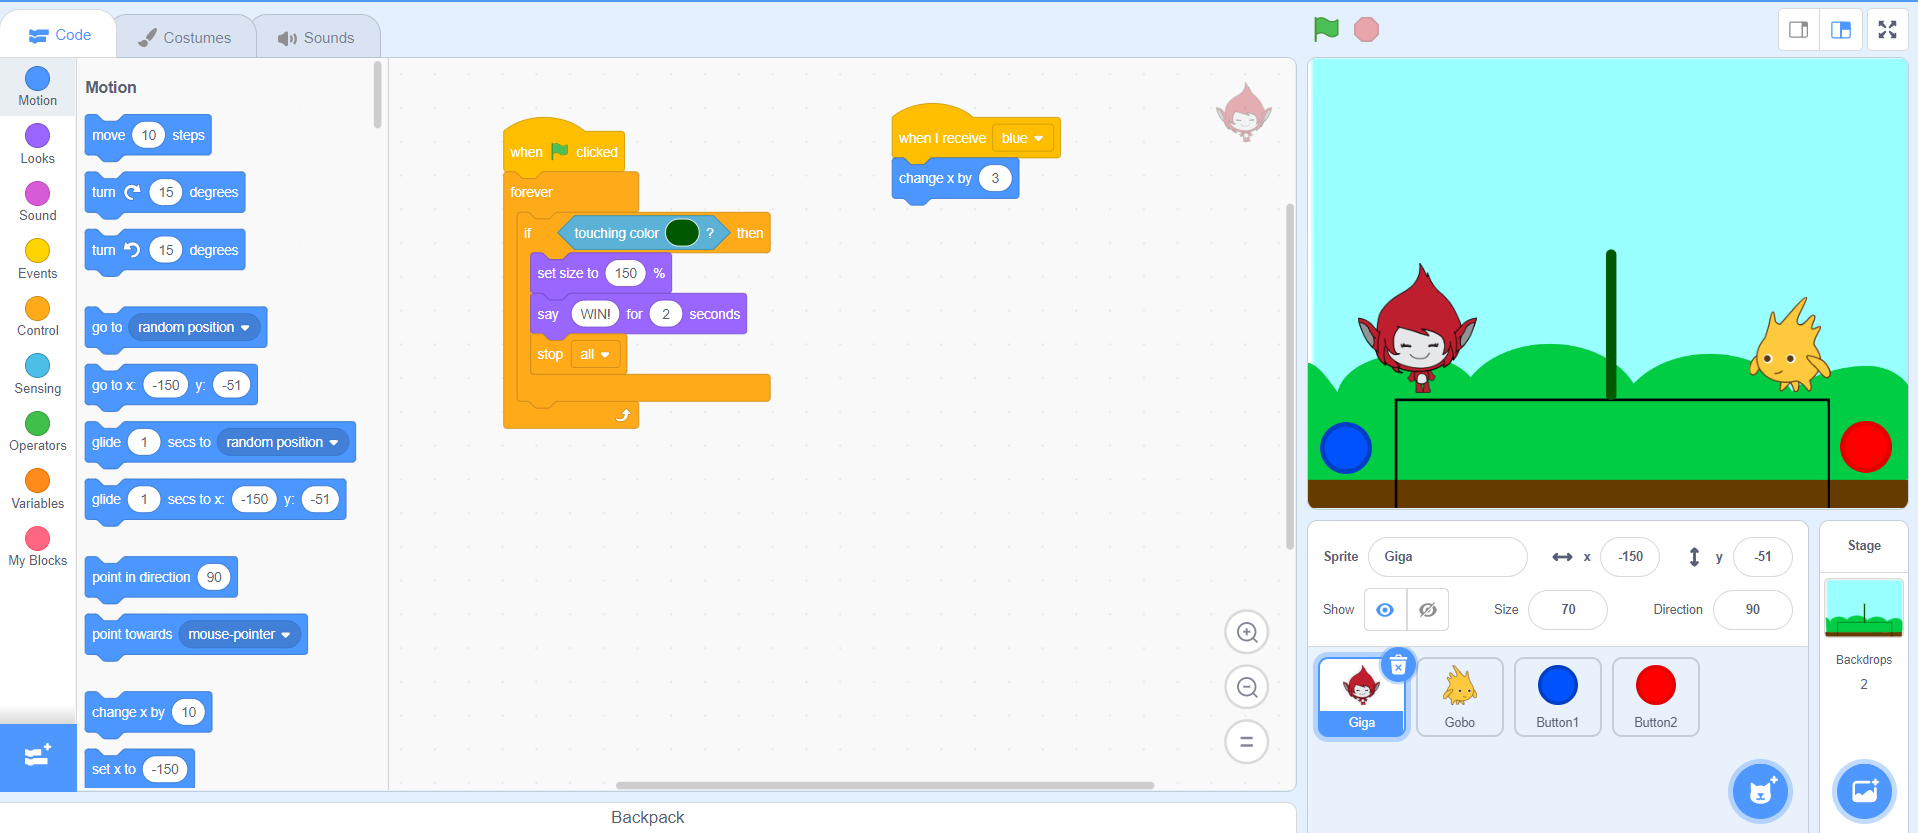
\includegraphics[width=1.0\linewidth,height=0.5\linewidth]{fig030019.png}
   \caption{Instructions for victory}
\label{fig030019}
\end{figure}

The last improvement that needs to be done to complete this character is to be placed in the starting position every time the game starts. In the blue section is the instruction that tells where to position the character.

\begin{figure}[H]
   \centering
   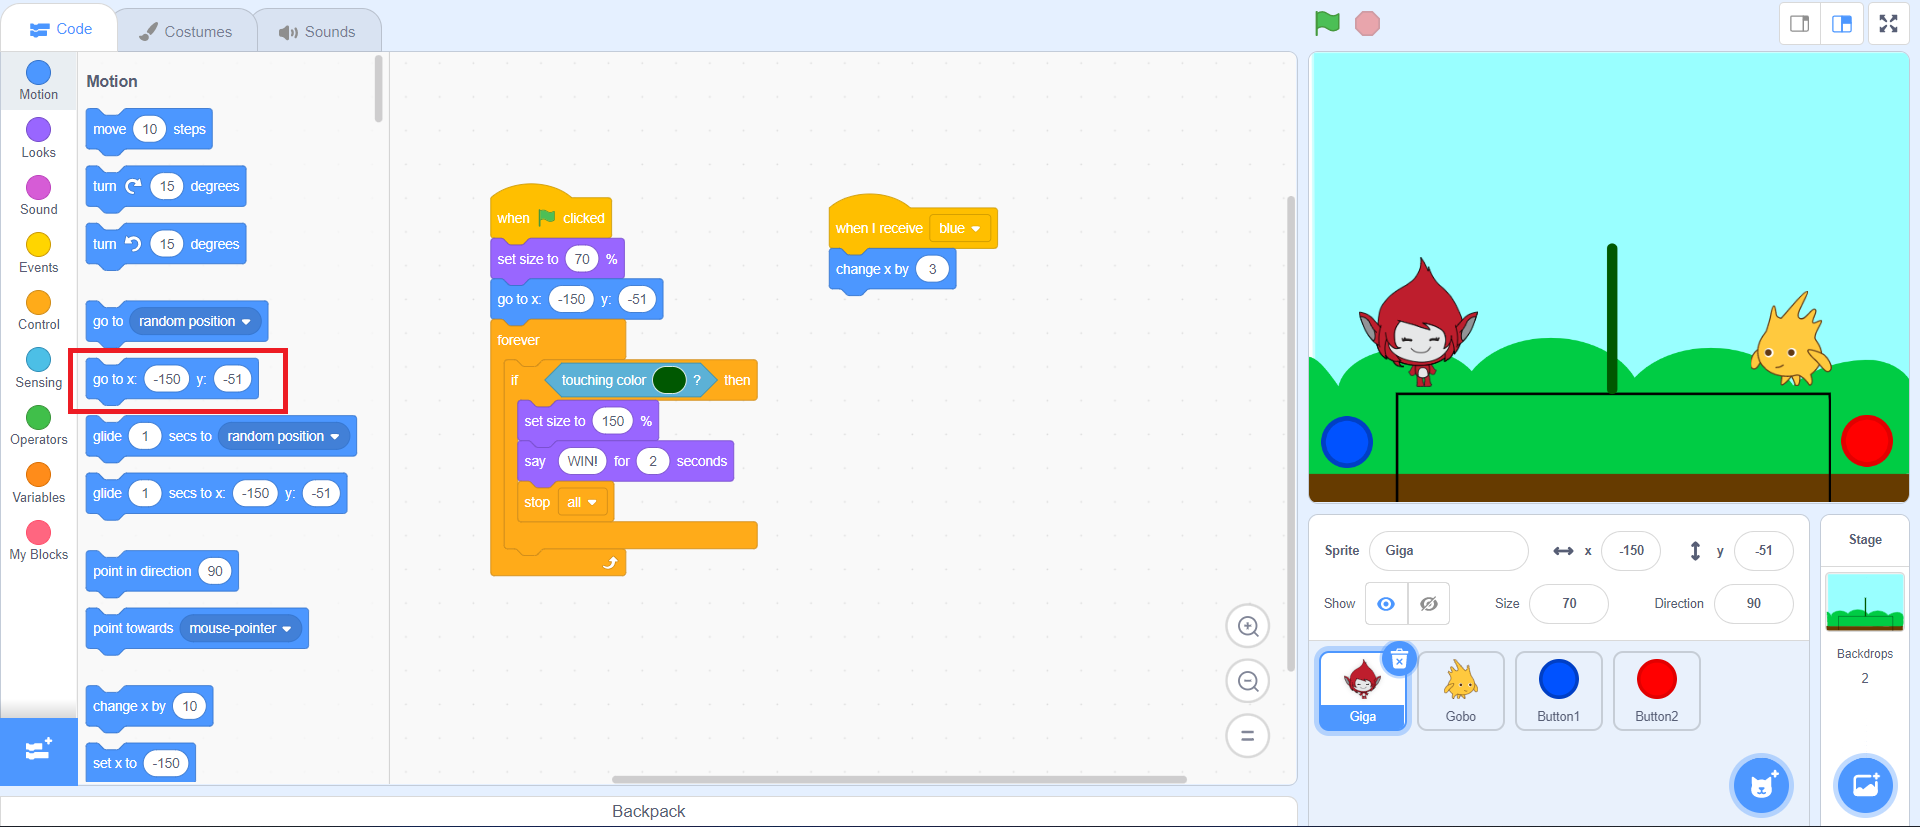
\includegraphics[width=1.0\linewidth,height=0.5\linewidth]{fig030020.png}
   \caption{Hero Positioning Instructions}
\label{fig030020}
\end{figure}

The final code of this character is:

\begin{figure}[H]
   \centering
   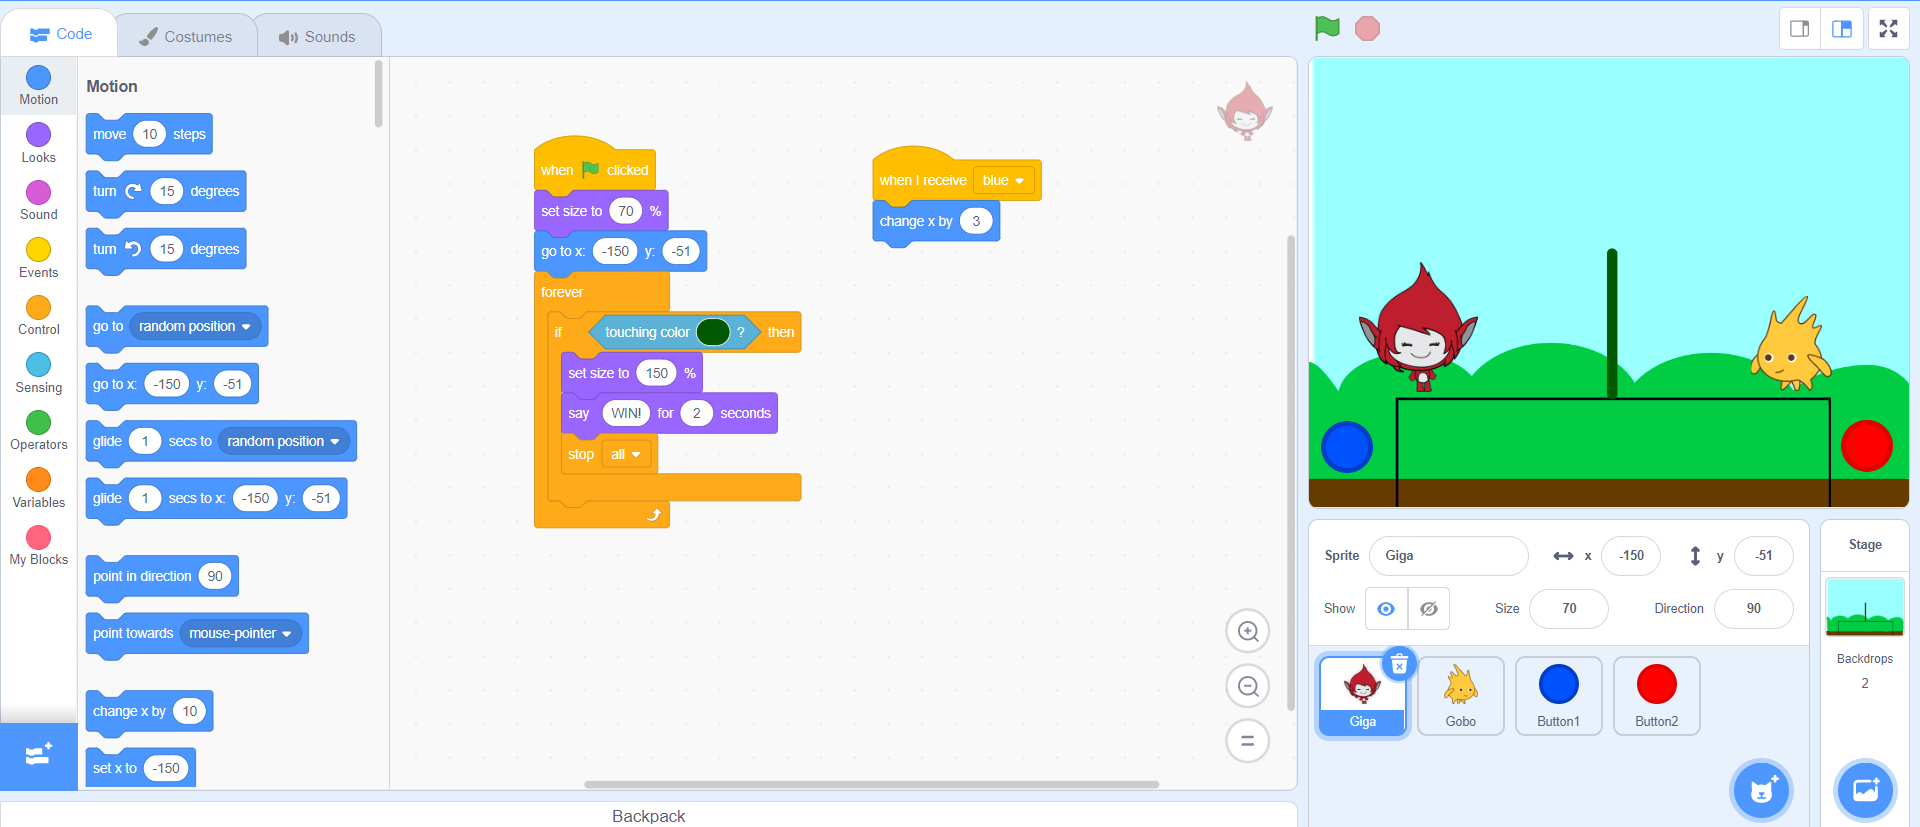
\includegraphics[width=1.0\linewidth,height=0.5\linewidth]{fig030021.png}
   \caption{Final code of left character}
\label{fig030021}
\end{figure}

Once that character is ready, it remains to add the instructions for defeating the other character as well. The code is similar. The only difference is in the starting coordinates.

\begin{figure}[H]
   \centering
   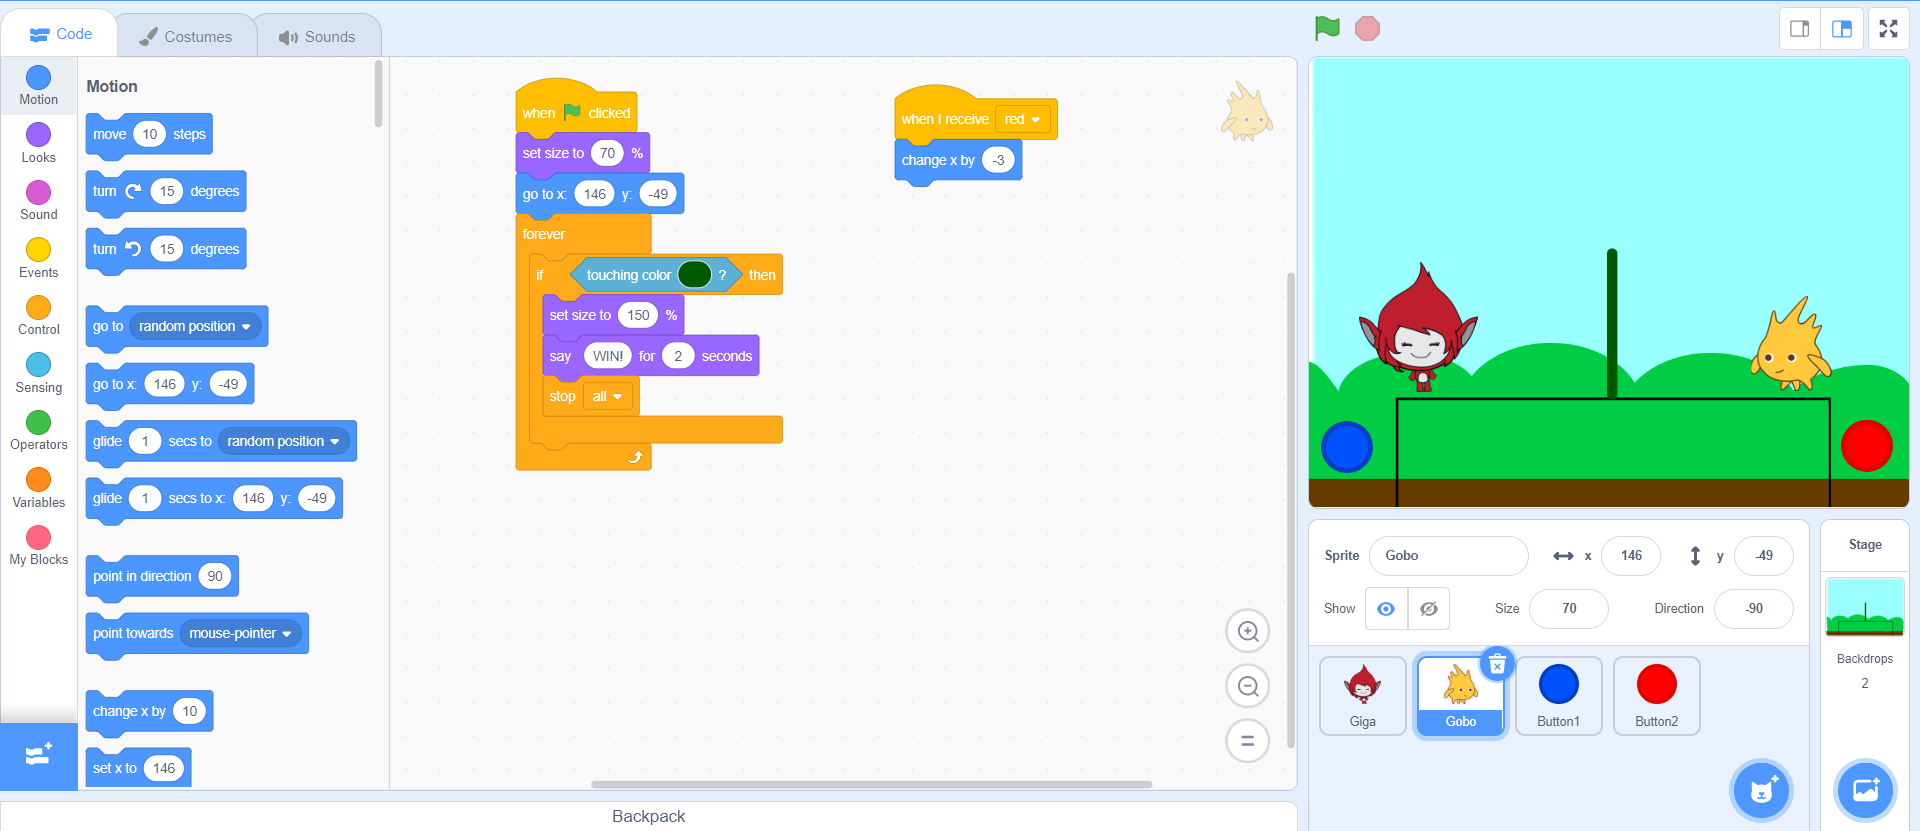
\includegraphics[width=1.0\linewidth,height=0.5\linewidth]{fig030022.png}
   \caption{Final code of the right character}
\label{fig030022}
\end{figure}

It's time to have fun with friends and compete to see which character will reach the finish line faster.
